\setchapterimage{figure/Chapter5封面图}
\setchapterintro{}
\chapter{一般理论}\label{chap:一般理论}

\section{Picard 存在唯一性定理}\label{sec:Picard存在唯一性定理}

考虑一阶微分方程
\[
	\dfrac{\dd x}{\dd t}=f(t,x)
\]
以及初值问题
\[
	\dfrac{\dd x}{\dd t}=f(t,x),
	\qquad
	x(t_0)=x_0.
\]
设函数 $f(t,x)$ 在矩形区域
\[
	R=\bigl\{(t,x)\in\R^2:\abs{t-t_0}\leq a,\ \abs{x-x_0}\leq b\bigr\}
\]
上连续。

\begin{definition}\label{def:关于x的Lipschitz条件}
	若存在常数 $L>0$，使得对任意
	$(t,x_1),(t,x_2)\in R$，都有
	\[
		\abs{f(t,x_1)-f(t,x_2)}
		\leq L\abs{x_1-x_2},
	\]
	则称函数 $f(t,x)$ 在 $R$ 上关于变量 $x$ 满足
	\textbf{Lipschitz 条件}，并称 $L$ 为一个 Lipschitz 常数。
\end{definition}

\begin{theorem}[Picard 存在唯一性定理]\label{thm:Picard存在唯一性定理}
	设函数 $f(t,x)$ 在矩形区域 $R$ 上连续，并且关于变量 $x$
	满足 Lipschitz 条件。令
	\[
		M=\max_{(t,x)\in R}\abs{f(t,x)},
		\qquad
		h=\min\left\{a,\dfrac{b}{M}\right\},
	\]
	则初值问题
	\[
	\dfrac{\dd x}{\dd t}=f(t,x),
	\qquad
	x(t_0)=x_0.
	\]在区间
	\[
		I=[t_0-h,t_0+h]
	\]
	上存在唯一解。当 $M=0$ 时，约定取 $h=a$。
\end{theorem}

\begin{proof}
	只证明右半区间 $[t_0,t_0+h]$ 上的结论，左半区间上的证明完全相同。

	\noindent\textbf{第一步}\quad
	初值问题与积分方程
	\[
		x(t)=x_0+\int_{t_0}^{t}f\bigl(\tau,x(\tau)\bigr)\dd\tau
	\]
	等价。事实上，初值问题的解经积分后满足该积分方程；反过来，
	积分方程的连续解由微积分基本定理可知连续可微，并满足原初值问题。

	\noindent\textbf{第二步}\quad
	取
	\[
		\varphi_0(t)\equiv x_0,
	\]
	并递归定义 Picard 迭代函数
	\[
		\varphi_n(t)
		=x_0+\int_{t_0}^{t}
		f\bigl(\tau,\varphi_{n-1}(\tau)\bigr)\dd\tau,
		\qquad n=1,2,\ldots.
	\]
	用归纳法可知，每个 $\varphi_n$ 都在 $[t_0,t_0+h]$ 上有定义且连续，
	并且
	\[
		\abs{\varphi_n(t)-x_0}\leq b.
	\]
	事实上，结论对 $\varphi_0$ 显然成立。若对 $\varphi_k$ 成立，
	则 $(t,\varphi_k(t))\in R$，因而 $\varphi_{k+1}$ 有定义且连续，并且
	\[
		\begin{aligned}
			\abs{\varphi_{k+1}(t)-x_0}
			&\leq\int_{t_0}^{t}
			\abs{f\bigl(\tau,\varphi_k(\tau)\bigr)}\dd\tau\\
			&\leq M(t-t_0)
			\leq Mh
			\leq b.
		\end{aligned}
	\]

	\noindent\textbf{第三步}\quad
	证明函数序列 $\{\varphi_n\}$ 一致收敛。考虑伸缩级数
	\[
		\varphi_0(t)
		+\sum_{k=1}^{\infty}
		\bigl(\varphi_k(t)-\varphi_{k-1}(t)\bigr),
	\]
	它的第 $n$ 个部分和正是 $\varphi_n(t)$。由 Lipschitz 条件和归纳法可得
	\[
		\abs{\varphi_k(t)-\varphi_{k-1}(t)}
		\leq
		\dfrac{ML^{k-1}}{k!}(t-t_0)^k
		\leq
		\dfrac{ML^{k-1}h^k}{k!}.
	\]
	这里 $k=1$ 时结论由 $\abs{f(t,x_0)}\leq M$ 得到；若结论对 $k$
	成立，则
	\[
		\begin{aligned}
			\abs{\varphi_{k+1}(t)-\varphi_k(t)}
			&\leq L\int_{t_0}^{t}
			\abs{\varphi_k(\tau)-\varphi_{k-1}(\tau)}\dd\tau\\
			&\leq
			\dfrac{ML^k}{(k+1)!}(t-t_0)^{k+1}.
		\end{aligned}
	\]
	数项级数
	\[
		\sum_{k=1}^{\infty}\dfrac{ML^{k-1}h^k}{k!}
	\]
	收敛，故由 Weierstrass 判别法，上述函数项级数一致收敛。
	记 $\varphi_n\to\varphi$，则 $\varphi$ 连续，且
	$\abs{\varphi(t)-x_0}\leq b$。

	\noindent\textbf{第四步}\quad
	证明极限函数 $\varphi$ 满足积分方程。由 Lipschitz 条件，
	\[
		\abs{
			f\bigl(t,\varphi_n(t)\bigr)
			-f\bigl(t,\varphi(t)\bigr)
		}
		\leq L\abs{\varphi_n(t)-\varphi(t)},
	\]
	所以 $f(t,\varphi_n(t))$ 一致收敛于 $f(t,\varphi(t))$。在迭代式中
	令 $n\to\infty$，可以逐项取极限，得到
	\[
		\begin{aligned}
			\varphi(t)
			&=x_0+\lim_{n\to\infty}
			\int_{t_0}^{t}
			f\bigl(\tau,\varphi_{n-1}(\tau)\bigr)\dd\tau\\
			&=x_0+\int_{t_0}^{t}
			f\bigl(\tau,\varphi(\tau)\bigr)\dd\tau.
		\end{aligned}
	\]
	因此 $\varphi$ 是原初值问题的解。

	\noindent\textbf{第五步}\quad
	证明解的唯一性。设 $\varphi$ 和 $\psi$ 都是初值问题在
	$[t_0,t_0+h]$ 上的解，则
	\[
		\begin{aligned}
			\abs{\varphi(t)-\psi(t)}
			&\leq\int_{t_0}^{t}
			\abs{
				f\bigl(\tau,\varphi(\tau)\bigr)
				-f\bigl(\tau,\psi(\tau)\bigr)
			}\dd\tau\\
			&\leq L\int_{t_0}^{t}
			\abs{\varphi(\tau)-\psi(\tau)}\dd\tau.
		\end{aligned}
	\]
	令
	\[
		v(t)=\int_{t_0}^{t}
		\abs{\varphi(\tau)-\psi(\tau)}\dd\tau,
	\]
	则 $v(t)\geq0$，$v(t_0)=0$，并且
	\[
		v'(t)\leq Lv(t).
	\]
	于是
	\[
		\dfrac{\dd}{\dd t}
		\left(\mathrm{e}^{-L(t-t_0)}v(t)\right)\leq0.
	\]
	故 $\mathrm{e}^{-L(t-t_0)}v(t)\leq v(t_0)=0$。结合 $v(t)\geq0$
	可知 $v(t)\equiv0$，从而 $\varphi(t)\equiv\psi(t)$。
	左右两个半区间合并后，定理得证。
\end{proof}


\subsection*{有限维情形}

考虑 $n$ 维一阶微分方程组
\[
	\dfrac{\dd\vect{x}}{\dd t}
	=\vect{f}(t,\vect{x}),
	\qquad
	\vect{x}(t_0)=\vect{x}_0,
\]
其中
\[
	\vect{x}
	=\begin{pmatrix}
		x_1\\
		x_2\\
		\vdots\\
		x_n
	\end{pmatrix},
	\qquad
	\vect{f}
	=\begin{pmatrix}
		f_1\\
		f_2\\
		\vdots\\
		f_n
	\end{pmatrix}.
\]
在 $\R^n$ 上取一个固定的向量范数 $\norm{\cdot}$，并记
\[
	\Omega
	=\left\{
		(t,\vect{x})\in\R\times\R^n:
		\abs{t-t_0}\leq a,\ 
		\norm{\vect{x}-\vect{x}_0}\leq b
	\right\}.
\]

\begin{definition}\label{def:向量函数的Lipschitz条件}
	若存在常数 $L>0$，使得对任意
	$(t,\vect{x}),(t,\vect{y})\in\Omega$，都有
	\[
		\norm{
			\vect{f}(t,\vect{x})
			-\vect{f}(t,\vect{y})
		}
		\leq
		L\norm{\vect{x}-\vect{y}},
	\]
	则称 $\vect{f}(t,\vect{x})$ 在 $\Omega$ 上关于向量变量
	$\vect{x}$ 满足 \textbf{Lipschitz 条件}。
\end{definition}

\begin{theorem}[有限维 Picard 存在唯一性定理]
	\label{thm:有限维Picard存在唯一性定理}
	设向量函数
	$\vect{f}\colon\Omega\to\R^n$ 连续，并且关于 $\vect{x}$
	满足 Lipschitz 条件。令
	\[
		M=\max_{(t,\vect{x})\in\Omega}
		\norm{\vect{f}(t,\vect{x})},
		\qquad
		h=\min\left\{a,\dfrac{b}{M}\right\},
	\]
	则上述初值问题在区间
	\[
		I=[t_0-h,t_0+h]
	\]
	上存在唯一的向量值解
	$\vect{x}\in C^1(I,\R^n)$。当 $M=0$ 时，约定取 $h=a$。
\end{theorem}

\begin{proof}
	仍只证明右半区间 $[t_0,t_0+h]$ 上的结论。

	\noindent\textbf{第一步}\quad
	逐分量积分可知，初值问题等价于向量积分方程
	\[
		\vect{x}(t)
		=\vect{x}_0
		+\int_{t_0}^{t}
		\vect{f}\bigl(\tau,\vect{x}(\tau)\bigr)\dd\tau.
	\]

	\noindent\textbf{第二步}\quad
	定义 Picard 迭代函数
	\[
		\vect{\varphi}_0(t)\equiv\vect{x}_0,
	\]
	\[
		\vect{\varphi}_n(t)
		=\vect{x}_0
		+\int_{t_0}^{t}
		\vect{f}\bigl(\tau,\vect{\varphi}_{n-1}(\tau)\bigr)\dd\tau,
		\qquad n=1,2,\ldots.
	\]
	利用向量积分的范数估计并作归纳，有
	\[
		\begin{aligned}
			\norm{\vect{\varphi}_{k+1}(t)-\vect{x}_0}
			&\leq
			\int_{t_0}^{t}
			\norm{
				\vect{f}\bigl(\tau,\vect{\varphi}_k(\tau)\bigr)
			}\dd\tau\\
			&\leq M(t-t_0)
			\leq Mh
			\leq b.
		\end{aligned}
	\]
	因此每个 $\vect{\varphi}_n$ 都在该区间上有定义且连续，
	并且其图像始终位于 $\Omega$ 中。

	\noindent\textbf{第三步}\quad
	与一维情形相同，由 Lipschitz 条件归纳得到
	\[
		\norm{
			\vect{\varphi}_k(t)-\vect{\varphi}_{k-1}(t)
		}
		\leq
		\dfrac{ML^{k-1}}{k!}(t-t_0)^k
		\leq
		\dfrac{ML^{k-1}h^k}{k!}.
	\]
	数项级数
	\[
		\sum_{k=1}^{\infty}
		\dfrac{ML^{k-1}h^k}{k!}
	\]
	收敛，故向量函数项级数
	\[
		\vect{\varphi}_0(t)
		+\sum_{k=1}^{\infty}
		\bigl(
			\vect{\varphi}_k(t)-\vect{\varphi}_{k-1}(t)
		\bigr)
	\]
	一致收敛。记 $\vect{\varphi}_n\to\vect{\varphi}$，则
	$\vect{\varphi}$ 连续，并且
	\[
		\norm{\vect{\varphi}(t)-\vect{x}_0}\leq b.
	\]

	\noindent\textbf{第四步}\quad
	由 Lipschitz 条件，
	\[
		\norm{
			\vect{f}\bigl(t,\vect{\varphi}_n(t)\bigr)
			-\vect{f}\bigl(t,\vect{\varphi}(t)\bigr)
		}
		\leq
		L\norm{\vect{\varphi}_n(t)-\vect{\varphi}(t)}.
	\]
	所以
	$\vect{f}(t,\vect{\varphi}_n(t))$
	一致收敛于
	$\vect{f}(t,\vect{\varphi}(t))$。在迭代式中取极限，得到
	\[
		\vect{\varphi}(t)
		=\vect{x}_0
		+\int_{t_0}^{t}
		\vect{f}\bigl(\tau,\vect{\varphi}(\tau)\bigr)\dd\tau.
	\]
	因此 $\vect{\varphi}$ 是原初值问题的解。

	\noindent\textbf{第五步}\quad
	设 $\vect{\varphi}$ 与 $\vect{\psi}$ 是两个解，则
	\[
		\norm{\vect{\varphi}(t)-\vect{\psi}(t)}
		\leq
		L\int_{t_0}^{t}
		\norm{\vect{\varphi}(\tau)-\vect{\psi}(\tau)}\dd\tau.
	\]
	令
	\[
		v(t)=
		\int_{t_0}^{t}
		\norm{\vect{\varphi}(\tau)-\vect{\psi}(\tau)}\dd\tau,
	\]
	则 $v(t)\geq0$，$v(t_0)=0$，并且 $v'(t)\leq Lv(t)$。于是
	\[
		\dfrac{\dd}{\dd t}
		\left(\mathrm{e}^{-L(t-t_0)}v(t)\right)\leq0,
	\]
	从而 $v(t)\equiv0$，即
	$\vect{\varphi}(t)\equiv\vect{\psi}(t)$。
	左半区间上的证明相同，故初值问题在 $I$ 上的解存在且唯一。
\end{proof}

\noindent\textbf{注 5.1}\quad
在实际应用中，直接验证关于 $x$ 的 Lipschitz 条件有时并不方便。
若偏导数 $\dfrac{\partial f}{\partial x}$ 在矩形区域 $R$ 上连续，则它在
$R$ 上有界。取
\[
L=\max_{(t,x)\in R}
\abs{\dfrac{\partial f}{\partial x}(t,x)},
\]
由 Lagrange 中值定理可得
\[
\abs{f(t,x_1)-f(t,x_2)}
\leq L\abs{x_1-x_2},
\]
故 $f$ 关于 $x$ 满足 Lipschitz 条件。

\noindent\textbf{注 5.2}\quad
对于一阶线性方程
\[
\dfrac{\dd x}{\dd t}=a(t)x+f(t),
\]
若 $a(t)$ 与 $f(t)$ 在区间 $[\alpha,\beta]$ 上连续，则 Picard
存在唯一性定理的条件成立。由于方程右端对 $x$ 没有定义域限制，
Picard 迭代函数可在整个区间 $[\alpha,\beta]$ 上逐次构造并一致收敛，
所以任意以 $t_0\in[\alpha,\beta]$ 为初始时刻的解都可延拓到整个区间。

\noindent\textbf{注 5.3}\quad
Picard 存在唯一性定理不仅给出解的存在唯一性，而且给出了构造近似解的方法。
若 $\varphi$ 是初值问题在 $[t_0-h,t_0+h]$ 上的解，则第 $n$ 次
Picard 近似满足误差估计
\[
\abs{\varphi_n(t)-\varphi(t)}
\leq
\dfrac{ML^n}{(n+1)!}h^{n+1}.
\]
这一估计可由
$\abs{\varphi_0(t)-\varphi(t)}\leq M\abs{t-t_0}$
和 Lipschitz 条件递推得到。

\subsection*{Picard迭代的压缩映射解释}
\phantomsection\label{sec:picard-contraction}
前面的 Picard 证明利用阶乘估计证明逐次逼近序列收敛。若适当缩小时间区间，还可将相应的积分算子看作压缩映射，从而由压缩映射定理得到解的存在性与唯一性。

\begin{definition}
度量空间 $(M,d)$ 中，
若映射 $A:M\to M$ 满足存在同一个常数 $0\leq\lambda<1$，使
\[
 d(Ax,Ay)\leq\lambda d(x,y)
\]
 对所有 $x,y\in M$ 成立，则称它为压缩映射。
满足 $Ax=x$ 的点称不动点。
\end{definition}
\begin{theorem}[压缩映射定理]\label{thm:arnold-banach}
非空完备度量空间上的压缩映射有唯一不动点 $x_*$。
任意初值的迭代 $x_{n+1}=Ax_n$ 收敛到它，并有
\[
 \begin{aligned}
 d(x_n,x_*)&\leq\frac{\lambda^n}{1-\lambda}d(x_0,Ax_0),\\
 d(x,x_*)&\leq\frac{d(x,Ax)}{1-\lambda}.
\end{aligned}
\]
\end{theorem}
\begin{proof}
\textbf{第一步：构造 Cauchy 序列。}
固定 $x_0\in M$，令 $x_{n+1}=Ax_n$，记 $d_0=d(x_1,x_0)$。
反复应用压缩条件，得到
$d(x_{j+1},x_j)\leq\lambda^jd_0$。
对 $m>n$，三角不等式和几何级数给出
\[
 \begin{aligned}
 d(x_m,x_n)&\leq\sum_{j=n}^{m-1}d(x_{j+1},x_j)\\
 &\leq d_0\sum_{j=n}^{m-1}\lambda^j\\
 &\leq\frac{\lambda^n}{1-\lambda}d_0.
\end{aligned}
\]
右端不依赖 $m$，且随 $n\to\infty$ 趋于零，所以这是 Cauchy 序列。
由完备性，存在 $x_*\in M$ 使 $x_n\to x_*$。

\textbf{第二步：验证不动点并证明唯一性。}
由压缩估计，$A$ 连续，故
\[
 Ax_*=\lim Ax_n=\lim x_{n+1}=x_*.
\]
若 $Ay_*=y_*$，则
\[
 d(x_*,y_*)\leq\lambda d(x_*,y_*).
\]
由于 $1-\lambda>0$，只能有 $d(x_*,y_*)=0$，即 $x_*=y_*$。

\textbf{第三步：误差估计。}
让第一步的不等式中 $m\to\infty$，便得到迭代误差界。
对任意近似点 $x$，另由
\[
 \begin{aligned}
 d(x,x_*)&\leq d(x,Ax)+d(Ax,Ax_*)\\
 &\leq d(x,Ax)+\lambda d(x,x_*)
\end{aligned}
\]
移项得到残差界 $d(x,x_*)\leq d(x,Ax)/(1-\lambda)$。
\end{proof}
只要求 $d(Ax,Ay)<d(x,y)$ 不够。例如
$A(x)=\log(1+e^x)$ 在 $\R$ 上满足 $0<A'(x)<1$，却始终 $A(x)>x$ 而没有不动点。
因此，压缩条件中必须存在一个对所有点都适用且严格小于 1 的常数。

\begin{proposition}[Picard 算子]
在矩形 $|t-t_0|\leq a,\ |x-x_0|\leq b$ 上，设 $|f|\leq M$，且 $f$ 关于 $x$
的 Lipschitz 常数为 $L$。取 $h\leq a$，$Mh\leq b$、$Lh<1$。
则
\[
 (Au)(t)=x_0+\int_{t_0}^tf(s,u(s))\,\dd s
\]
在连续函数的闭集 $\{u:\|u-x_0\|_\infty\leq b\}$ 上为压缩映射。
\end{proposition}
\begin{proof}
令 $J=[t_0-h,t_0+h]$，在 $C(J,\R^n)$ 上取一致范数。
连续函数列若依一致范数 Cauchy，便一致收敛到连续函数，故该空间完备。
集合 $\mathcal M=\{u:\|u-x_0\|_\infty\leq b\}$ 是闭集，且包含常函数 $u=x_0$，
因此是非空完备度量空间。

若 $u\in\mathcal M$，则所有 $(t,u(t))$ 都在给定矩形内，所以积分有定义，且
\[
 |(Au)(t)-x_0|\leq\left|\int_{t_0}^t M\,ds\right|
 \leq Mh\leq b.
\]
这证明 $A\mathcal M\subset\mathcal M$。
对任意 $u,w\in\mathcal M$，Lipschitz 条件给出
\[
 |(Au)(t)-(Aw)(t)|\leq L|t-t_0|\|u-w\|_\infty.
\]
取上确界得 
\[
 \|Au-Aw\|_\infty\leq Lh\|u-w\|_\infty.
\]
由于 $Lh<1$，压缩映射定理适用。
其不动点满足积分方程，右端连续，所以对时间可微，微分后满足原初值问题。
反过来，每个处于此矩形内的解积分后也是不动点，唯一性随之成立。
\end{proof}

\section{Peano 存在性定理}\label{sec:Peano存在性定理}

\begin{definition}\label{def:一致有界与等度连续}
	函数族 $\mathcal{F}=\{f(t)\}$ 称为在有界闭区间
	$[\alpha,\beta]$ 上\textbf{一致有界}的，如果存在常数 $M_0>0$，
	使得对任意 $f\in\mathcal{F}$，都有
	\[
		\abs{f(t)}\leq M_0,
		\qquad t\in[\alpha,\beta].
	\]

	函数族 $\mathcal{F}$ 称为在 $[\alpha,\beta]$ 上\textbf{等度连续}的，
	如果对任意 $\eps>0$，存在只与 $\eps$ 有关的常数
	$\delta(\eps)>0$，使得对任意 $f\in\mathcal{F}$，只要
	$t,s\in[\alpha,\beta]$ 且 $\abs{t-s}<\delta(\eps)$，就有
	\[
		\abs{f(t)-f(s)}<\eps.
	\]
\end{definition}

一致有界的函数族中的每个函数都是有界函数，等度连续的函数族中的每个函数
都是一致连续函数，但反之一般不成立。

\begin{lemma}(Ascoli--Arzelà 引理)\label{lem:AscoliArzela引理}
	定义在有界闭区间 $[\alpha,\beta]$ 上的一致有界且等度连续的无穷函数族
	$\mathcal{F}$，必含有一个在 $[\alpha,\beta]$ 上一致收敛的函数序列。
\end{lemma}

\begin{proof}
	由一致有界性，存在 $M_0>0$，使得对任意 $f\in\mathcal{F}$，
	\[
		\abs{f(t)}\leq M_0,
		\qquad t\in[\alpha,\beta].
	\]
	因此 $\mathcal{F}$ 中所有函数的图像都位于矩形区域
	\[
		R_0
		=\left\{
			(t,x)\in\R^2:
			\alpha\leq t\leq\beta,\ 
			-M_0\leq x\leq M_0
		\right\}
	\]
	内。

	取 $s_1=\dfrac{M_0}{2}$。由等度连续性，存在
	$\delta_1>0$，使得对任意 $f\in\mathcal{F}$，当
	$\abs{t-\bar t}<\delta_1$ 时都有
	\[
		\abs{f(t)-f(\bar t)}\leq s_1.
	\]
	用平行于坐标轴的直线将 $R_0$ 分成有限多个高为 $s_1$、
	宽不超过 $\delta_1$ 的小矩形。每个函数的图像在任一竖直长条内
	至多经过两个相邻的小矩形，因而被包含在某个高为 $2s_1$ 的多边形中。
	这样的多边形只有有限多个，所以至少有一个多边形 $S_1$
	包含 $\mathcal{F}$ 中无穷多个函数的图像，记这些函数组成的子族为
	$\mathcal{F}_1$。

	再取 $s_2=\dfrac{M_0}{2^2}$。对 $\mathcal{F}_1$ 重复上述构造，
	可在 $S_1$ 内找到一个高为 $2s_2$ 的多边形 $S_2$，其中仍包含
	$\mathcal{F}_1$ 中无穷多个函数的图像，记相应的无穷子族为
	$\mathcal{F}_2$。这一嵌套构造如图所示。

\begin{center}
	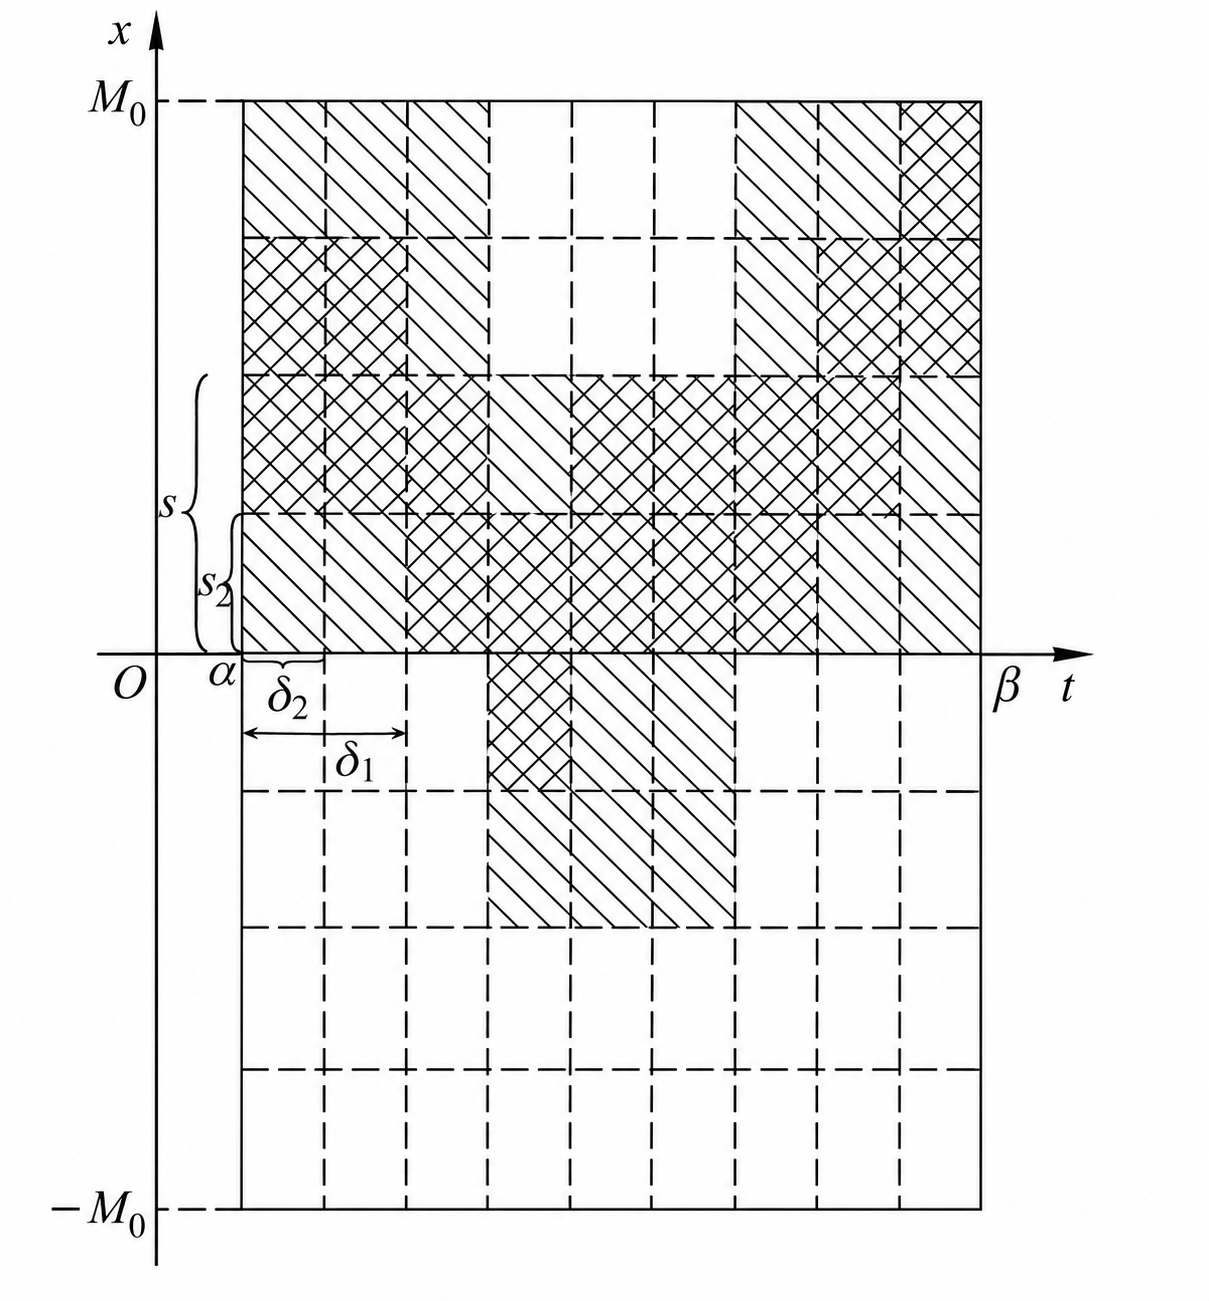
\includegraphics[width=0.5\linewidth]{figure/111}
\end{center}

	一般地，令
	\[
		s_k=\dfrac{M_0}{2^k}.
	\]
	可依次得到多边形 $S_k$ 及无穷函数族 $\mathcal{F}_k$，使得
	\[
		\mathcal{F}\supset\mathcal{F}_1
		\supset\cdots\supset\mathcal{F}_k\supset\cdots,
	\]
	并且对任意 $f_1^{(k)},f_2^{(k)}\in\mathcal{F}_k$，
	\[
		\abs{f_1^{(k)}(t)-f_2^{(k)}(t)}
		\leq2s_k
		=\dfrac{M_0}{2^{k-1}},
		\qquad t\in[\alpha,\beta].
	\]
	依次选取互不相同的 $f_k\in\mathcal{F}_k$。由于函数族逐层嵌套，
	对任意 $l\geq k$ 都有
	\[
		\abs{f_k(t)-f_l(t)}
		\leq\dfrac{M_0}{2^{k-1}},
		\qquad t\in[\alpha,\beta].
	\]
	故 $\{f_k\}$ 在 $[\alpha,\beta]$ 上一致满足 Cauchy 收敛准则，
	从而一致收敛。
\end{proof}

仍考虑初值问题
\[
	\dfrac{\dd x}{\dd t}=f(t,x),
	\qquad
	x(t_0)=x_0,
\]
但这里只要求 $f(t,x)$ 在矩形区域
\[
	R=\left\{
		(t,x)\in\R^2:
		\abs{t-t_0}\leq a,\ 
		\abs{x-x_0}\leq b
	\right\}
\]
上连续，不要求它关于 $x$ 满足 Lipschitz 条件。此时解仍然存在，
但不一定唯一。

\begin{theorem}(Peano 存在性定理)\label{thm:Peano存在性定理}
	若 $f(t,x)$ 在矩形区域 $R$ 上连续，则上述初值问题在区间
	\[
		I=[t_0-h,t_0+h]
	\]
	上至少有一个解，其中
	\[
		M=\max_{(t,x)\in R}\abs{f(t,x)},
		\qquad
		h=\min\left\{a,\dfrac{b}{M}\right\}.
	\]
	当 $M=0$ 时，约定取 $h=a$。
\end{theorem}

\begin{proof}
	\noindent\textbf{第一步：构造 Euler 折线。}\quad
	由
	\[
		\abs{x(t)-x_0}\leq M\abs{t-t_0}
	\]
	可知，为使所构造曲线的图像不越出 $R$，只需取
	$h=\min\{a,\dfrac{b}{M}\}$。

	任取正整数 $n$，令
	\[
		t_k=t_0+\dfrac{kh}{n},
		\qquad k=0,\pm1,\pm2,\ldots,\pm n,
	\]
	从而把区间 $I$ 分成 $2n$ 等份。从点
	$P_0=(t_0,x_0)$ 出发，以斜率 $f(t_0,x_0)$ 作直线段至
	$t=t_1$，记其端点为 $P_1=(t_1,x_1)$；再从 $P_1$ 出发，
	以斜率 $f(t_1,x_1)$ 作下一段。如此继续，得到
	\[
		x_{k+1}
		=x_k+f(t_k,x_k)(t_{k+1}-t_k),
		\qquad k=0,1,\ldots,n-1.
	\]
	向左作完全相同的构造，即得到整段 Euler 折线。

	\begin{figure}[htbp]
		\centering
		\begin{tikzpicture}[x=1.05cm,y=1cm,>=Stealth]
			\draw[->] (-4.25,0)--(4.45,0) node[right] {$t$};
			\draw[->] (0,-2.85)--(0,2.9) node[above] {$x$};
			\draw[thick] (-3.6,-2.3) rectangle (3.6,2.3);
			\draw[gray] (-2.35,-2.3)--(-2.35,2.3);
			\draw[gray] (2.35,-2.3)--(2.35,2.3);
			\draw[gray] (0,0)--(2.35,2.3);
			\draw[gray] (0,0)--(2.35,-2.3);
			\draw[gray] (0,0)--(-2.35,2.3);
			\draw[gray] (0,0)--(-2.35,-2.3);

			\draw[very thick]
				(0,0)
				--(0.62,0.48)
				--(1.18,0.83)
				--(1.72,0.95)
				--(2.35,1.28);
			\foreach \x/\y/\name in
				{0/0/P_0,0.62/0.48/P_1,1.18/0.83/P_2,1.72/0.95/P_3}
				{\fill (\x,\y) circle (1.3pt);
				 \node[above left] at (\x,\y) {$\name$};}
			\foreach \x/\y/\lab in
				{0.62/0.48/t_1,1.18/0.83/t_2,1.72/0.95/t_3}
				{\draw[dashed,gray] (\x,0)--(\x,\y);
				 \node[below] at (\x,0) {$\lab$};}

			\node[below left] at (0,0) {$(t_0,x_0)$};
			\node[left] at (-0.08,2.3) {$x_0+b$};
			\node[left] at (-0.08,-2.3) {$x_0-b$};
			\node[below] at (-3.6,0) {$t_0-a$};
			\node[below] at (3.6,0) {$t_0+a$};
		\end{tikzpicture}
		\caption{Euler 折线的构造}
		\label{fig:Euler折线构造}
	\end{figure}

	记所构造的折线函数为 $\varphi_n(t)$。对
	$s=0,1,\ldots,n-1$，它可写成
	\[
		\varphi_n(t)=
		\begin{cases}
			x_0+\displaystyle\sum_{k=0}^{s-1}
			f(t_k,x_k)(t_{k+1}-t_k)
			+f(t_s,x_s)(t-t_s),
			& t\in[t_s,t_{s+1}],\\[1.2em]
			x_0+\displaystyle\sum_{k=-s+1}^{0}
			f(t_k,x_k)(t_{k-1}-t_k)
			+f(t_{-s},x_{-s})(t-t_{-s}),
			& t\in(t_{-s-1},t_{-s}].
		\end{cases}
	\]
	当求和的下限大于上限时，约定该和为零。

	\noindent\textbf{第二步：证明 Euler 折线序列收敛。}\quad
	对任意 $n$，$\varphi_n$ 的图像始终位于 $R$ 内，故
	$\{\varphi_n\}$ 一致有界。每一段折线的斜率绝对值都不超过 $M$，
	因此对任意 $t,s\in I$，
	\[
		\abs{\varphi_n(t)-\varphi_n(s)}
		\leq M\abs{t-s}.
	\]
	所以 $\{\varphi_n\}$ 等度连续。由引理
	\ref{lem:AscoliArzela引理}，存在子序列
	$\{\varphi_{n_k}\}$ 在 $I$ 上一致收敛。记
	\[
		\varphi_{n_k}(t)\longrightarrow\varphi(t),
		\qquad t\in I.
	\]

	\noindent\textbf{第三步：证明 Euler 折线满足近似积分方程。}\quad
	只在 $[t_0,t_0+h]$ 上证明，左半区间完全相同。若
	$t\in[t_s,t_{s+1}]$，则对 $k=0,1,\ldots,s-1$，令
	\[
		d_n(k)
		=\int_{t_k}^{t_{k+1}}
		\left[
			f(t_k,x_k)-f\bigl(\tau,\varphi_n(\tau)\bigr)
		\right]\dd\tau,
	\]
	并令
	\[
		d_n^*(t)
		=\int_{t_s}^{t}
		\left[
			f(t_s,x_s)-f\bigl(\tau,\varphi_n(\tau)\bigr)
		\right]\dd\tau.
	\]
	于是利用积分的可加性可得
	\[
		\varphi_n(t)
		=x_0+\int_{t_0}^{t}
		f\bigl(\tau,\varphi_n(\tau)\bigr)\dd\tau
		+\sigma_n(t),
	\]
	其中
	\[
		\sigma_n(t)
		=\sum_{k=0}^{s-1}d_n(k)+d_n^*(t).
	\]

	下面证明 $\sigma_n\to0$。由于 $f$ 在紧集 $R$ 上一致连续，
	对任意 $\eps>0$，存在 $\delta>0$，使得当
	\[
		\abs{\tau-t_k}<\delta,
		\qquad
		\abs{\varphi_n(\tau)-x_k}<\delta
	\]
	时，有
	\[
		\abs{
			f(t_k,x_k)-f\bigl(\tau,\varphi_n(\tau)\bigr)
		}
		<\dfrac{\eps}{h}.
	\]
	当 $n$ 充分大时，
	\[
		\abs{t_{k+1}-t_k}
		=\dfrac{h}{n}<\delta,
	\]
	并且在每个小区间上
	\[
		\abs{\varphi_n(\tau)-x_k}
		\leq M\abs{\tau-t_k}
		\leq\dfrac{Mh}{n}<\delta.
	\]
	于是
	\[
		\abs{d_n(k)}<\dfrac{\eps}{n},
		\qquad
		\abs{d_n^*(t)}<\dfrac{\eps}{n}.
	\]
	因为 $s\leq n-1$，所以
	\[
		\abs{\sigma_n(t)}
		<\dfrac{s}{n}\eps+\dfrac{\eps}{n}
		\leq\eps.
	\]
	故 $\sigma_n(t)\to0$，而且收敛关于 $t$ 是一致的。

	\noindent\textbf{第四步：取极限。}\quad
	由 $\varphi_{n_k}\to\varphi$ 的一致收敛以及 $f$ 在 $R$ 上的一致连续性，
	\[
		f\bigl(t,\varphi_{n_k}(t)\bigr)
		\longrightarrow
		f\bigl(t,\varphi(t)\bigr)
	\]
	也一致成立。在近似积分方程中令 $k\to\infty$，得到
	\[
		\varphi(t)
		=x_0+\int_{t_0}^{t}
		f\bigl(\tau,\varphi(\tau)\bigr)\dd\tau,
		\qquad t\in I.
	\]
	因此 $\varphi$ 满足原初值问题的等价积分方程，从而是原初值问题的解。
\end{proof}

从几何上看，Euler 折线法给出了一种用折线逼近积分曲线的方法。

\begin{definition}\label{def:epsilon逼近解}
	定义在区间 $[\alpha,\beta]$ 上的函数 $x=\varphi(t)$
	称为上述初值问题在该区间上的一个 \textbf{$\eps$-逼近解}，如果
	$\varphi(t_0)=x_0$，并且满足：
	\begin{enumerate}
		\item $\varphi$ 在 $[\alpha,\beta]$ 上连续，除有限多个点外处处
			连续可微，并且在这些分点处的左、右导数都存在；
		\item 对任意 $t\in[\alpha,\beta]$，点
			$(t,\varphi(t))$ 都位于矩形区域 $R$ 内；
		\item 对任意 $t\in[\alpha,\beta]$，
			\[
				\abs{
					\dfrac{\dd\varphi(t)}{\dd t}
					-f\bigl(t,\varphi(t)\bigr)
				}\leq\eps.
			\]
	\end{enumerate}
	在不可微的分点处，若 $t\neq\beta$，上式中的导数取右导数；
	当 $t=\beta$ 时取左导数。
\end{definition}

\begin{proposition}\label{prop:Peano条件下epsilon逼近解的存在性}
	若 $f(t,x)$ 在矩形区域 $R$ 上连续，则对任意 $\eps>0$，
	初值问题在区间 $I=[t_0-h,t_0+h]$ 上存在 $\eps$-逼近解。
	由 Euler 折线得到的逼近解在右半区间上还满足
	\[
		\abs{\varphi(t)-\varphi(s)}
		\leq M\abs{t-s},
		\qquad t,s\in[t_0,t_0+h],
	\]
	其中
	\[
		h=\min\left\{a,\dfrac{b}{M}\right\},
		\qquad
		M=\max_{(t,x)\in R}\abs{f(t,x)}.
	\]
\end{proposition}

\subsection*{唯一性条件下的Euler折线}
Peano 定理利用紧性从 Euler 折线中抽取收敛子列。若另有 Lipschitz 条件，则第~\ref{sec:picard-contraction}~节的残差估计还能控制整个近似序列。
必要时缩小共同存在区间，仍记其半长为 $h$，并使 $Lh<1$。在该区间的连续函数闭集上，令
\[
 (Au)(t)=x_0+\int_{t_0}^tf(s,u(s))\,ds.
\]
记初值问题的解为 $x$，则 $Ax=x$，且对任一留在该闭集内的近似曲线 $u$，
\[
 \|u-x\|_\infty\leq\|u-Au\|_\infty/(1-Lh).
\]
在 Peano 定理的证明中已经得到 Euler 折线 $u_n$ 满足
\[
 u_n=Au_n+\sigma_n,\qquad\|\sigma_n\|_\infty\longrightarrow0.
\]
代入残差估计，便有
\[
 \|u_n-x\|_\infty\leq\frac{\|\sigma_n\|_\infty}{1-Lh}\longrightarrow0.
\]
因此在这个共同小区间上，整个 Euler 折线序列均一致收敛到解，而不只是某个子序列。

\section{解的延拓}\label{sec:解的延拓}

前面所得的存在性定理只保证初值问题在初始点附近有解。现在讨论：
已经得到的局部解能否继续向两端延伸，以及它最终能延伸到什么地方。

设 $f(t,x)$ 在开区域 $G\subset\R^2$ 内连续，$x=\varphi(t)$
是方程
\[
	\dfrac{\dd x}{\dd t}=f(t,x)
\]
在闭区间 $[\alpha,\beta]$ 上的一个解，并且其图像位于 $G$ 内。
由于
\[
	Q=\bigl(\beta,\varphi(\beta)\bigr)\in G,
\]
可在 $Q$ 的附近取一个完全落在 $G$ 内的小矩形。由定理
\ref{thm:Peano存在性定理}，
存在 $h_1>0$，使初值问题
\[
	\dfrac{\dd x}{\dd t}=f(t,x),
	\qquad x(\beta)=\varphi(\beta)
\]
在 $[\beta-h_1,\beta+h_1]$ 上有解 $x=\varphi_1(t)$。
同理，在左端点处存在 $h_2>0$ 以及定义在
$[\alpha-h_2,\alpha+h_2]$ 上的解 $x=\varphi_2(t)$，满足
$\varphi_2(\alpha)=\varphi(\alpha)$。于是分段函数
\[
	\psi(t)=
	\begin{cases}
		\varphi_2(t), & t\in[\alpha-h_2,\alpha],\\
		\varphi(t),   & t\in[\alpha,\beta],\\
		\varphi_1(t), & t\in[\beta,\beta+h_1]
	\end{cases}
\]
仍是原方程的解，并把 $\varphi$ 延伸到了更大的区间
$[\alpha-h_2,\beta+h_1]$ 上。几何上，这相当于在原积分曲线的两个端点
继续接上新的积分曲线段。

\begin{figure}[htbp]
	\centering
	\begin{tikzpicture}[x=1.05cm,y=1cm,>=Stealth]
		\draw[->] (-0.45,0)--(8.2,0) node[right] {$t$};
		\draw[->] (0,-0.45)--(0,4.65) node[above] {$x$};

		\draw[thick]
			(0.75,0.72)
			.. controls (0.22,1.45) and (0.58,3.38) .. (1.66,3.94)
			.. controls (2.75,4.51) and (4.62,4.17) .. (5.85,4.34)
			.. controls (7.06,4.50) and (7.67,3.67) .. (7.50,2.64)
			.. controls (7.32,1.52) and (6.45,0.67) .. (5.25,0.51)
			.. controls (3.68,0.30) and (1.60,0.16) .. cycle;
		\node at (6.72,3.78) {$G$};

		\draw[gray] (1.30,0.82) rectangle (2.78,2.25);
		\draw[gray] (2.15,1.07) rectangle (3.62,2.67);
		\draw[gray] (3.05,1.43) rectangle (4.55,3.10);
		\draw[gray] (4.05,1.75) rectangle (5.55,3.43);
		\draw[gray] (4.92,2.05) rectangle (6.43,3.70);

		\draw[very thick]
			(1.30,1.18)
			.. controls (2.17,1.43) and (2.58,1.95) .. (3.42,2.14)
			.. controls (4.12,2.30) and (4.74,2.58) .. (5.55,2.91)
			.. controls (5.91,3.06) and (6.18,3.15) .. (6.43,3.20);

		\fill (3.42,2.14) circle (1.5pt)
			node[above left] {$P=(t_0,x_0)$};
		\fill (5.55,2.91) circle (1.5pt)
			node[above left] {$Q$};

		\foreach \u/\v/\lab in
			{1.30/1.18/{\alpha-h_2},2.15/1.42/{\alpha},3.42/2.14/{t_0},5.55/2.91/{\beta},6.43/3.20/{\beta+h_1}}
			{
				\draw[dashed,gray] (\u,0)--(\u,\v);
				\node[below] at (\u,0) {$\lab$};
			}
	\end{tikzpicture}
	\caption{解的延拓}
	\label{fig:解的延拓}
\end{figure}

\begin{definition}\label{def:解的延拓与饱和解}
	设 $x=\varphi(t)$ 与 $x=\psi(t)$ 分别是定义在区间 $J_1,J_2$
	上的解。若 $J_1\subset J_2$，且 $\psi(t)=\varphi(t)$ 对所有
	$t\in J_1$ 成立，则称 $\psi$ 是 $\varphi$ 在 $J_2$ 上的
	\textbf{延拓}。若一个解不能再延拓到任何更大的区间，则称它为
	\textbf{饱和解}或\textbf{极大解}。
\end{definition}

\begin{theorem}[有限端点延拓判据]\label{thm:有限端点延拓判据}
	设 $f(t,x)$ 在区域 $G$ 内有界，并且关于 $x$ 局部满足
	Lipschitz 条件。若初值问题的饱和解 $x=\varphi(t)$ 的最大存在
	区间为
	\[
		-\infty<\alpha<t<\beta<+\infty,
	\]
	则极限
	\[
		\varphi(\alpha+0)
		=\lim_{t\to\alpha^+}\varphi(t),
		\qquad
		\varphi(\beta-0)
		=\lim_{t\to\beta^-}\varphi(t)
	\]
	都存在，且
	\[
		\bigl(\alpha,\varphi(\alpha+0)\bigr),
		\qquad
		\bigl(\beta,\varphi(\beta-0)\bigr)
	\]
	均为 $G$ 的边界点。
\end{theorem}

\begin{proof}
	设 $\abs{f(t,x)}\leq M$。当
	$\alpha<t_2<t_1<\beta$ 时，由积分方程，
	\[
		\begin{aligned}
		\abs{\varphi(t_1)-\varphi(t_2)}
		&=\abs{\int_{t_2}^{t_1}
		f\bigl(t,\varphi(t)\bigr)\dd t}\\
		&\leq M\abs{t_1-t_2}.
		\end{aligned}
	\]
	因此当 $t_1,t_2\to\alpha^+$ 时，
	$\varphi(t_1)-\varphi(t_2)\to0$。由 Cauchy 收敛准则，
	$\varphi(\alpha+0)$ 存在；同理，
	$\varphi(\beta-0)$ 存在。

	若 $\bigl(\alpha,\varphi(\alpha+0)\bigr)$ 是 $G$ 的内点，则可由
	Picard 存在唯一性定理将解延拓到某个区间
	\[
		\alpha-h_*<t<\beta,
		\qquad h_*>0,
	\]
	这与 $(\alpha,\beta)$ 为最大存在区间矛盾。故
	$\bigl(\alpha,\varphi(\alpha+0)\bigr)$ 为 $G$ 的边界点；右端点的
	结论同理。
\end{proof}

沿选定的解分支不断重复上述过程，可以得到饱和解；严格地说，也可由极大原理
保证其存在。饱和解的存在区间必为开区间。事实上，若右端点 $b$ 有限且
属于其存在区间，则 $(b,\varphi(b))\in G$，由定理
\ref{thm:Peano存在性定理} 还可越过
$b$ 继续延拓，这与饱和性矛盾；左端点同理。

为刻画积分曲线与边界的接近程度，定义点 $(t_0,x_0)$ 到集合
$D\subset\R^2$ 的距离为
\[
	\rho\bigl((t_0,x_0),D\bigr)
	=\inf_{(t,x)\in D}
	\sqrt{(t-t_0)^2+(x-x_0)^2}.
\]

定理 \ref{thm:有限端点延拓判据} 的两个附加条件---$f$ 在整个
$G$ 内有界，以及最大存在区间的端点有限---在下面的结论中都不再要求。
相应地，下面只能断言积分曲线延拓到区域的边界；若该边界位于无穷远处，
并不意味着 $\varphi(t)$ 在某个有限端点有极限。

\begin{theorem}[解的延拓定理]\label{thm:解的延拓定理}
	设 $G$ 为 $\R^2$ 上的一个开区域，$f(t,x)$ 在 $G$ 内连续。
	并且关于 $x$ 局部满足 Lipschitz 条件。
	对于方程的任一饱和解 $x=\varphi(t)$，积分曲线
	$x=\varphi(t)$ 必能达到 $G$ 的边界。特别地，当 $G$ 为有界区域，
	且饱和解 $x=\varphi(t)$ 的存在区间为 $(a,b)$ 时，
	\[
		\lim_{t\to b^-}
		\rho\bigl((t,\varphi(t)),\partial G\bigr)=0,
		\qquad
		\lim_{t\to a^+}
		\rho\bigl((t,\varphi(t)),\partial G\bigr)=0.
	\]
\end{theorem}

\begin{proof}
	把饱和解 $\varphi(t)$ 的最大存在区间记为 $J$。只证明
	$t\to b^-$ 时的结论；$t\to a^+$ 时完全类似。令
	\[
		J_+=J\cap[t_0,+\infty).
	\]

	\noindent\textbf{情形 1}
	若 $J_+=[t_0,+\infty)$，即 $b=+\infty$，则积分曲线在 $G$ 内
	可以延拓到无穷，因而在无穷远处达到 $\partial G$。

	\noindent\textbf{情形 2}
	若 $J_+=[t_0,b)$ 且 $b<+\infty$，则只需证明
	\[
		\lim_{t\to b^-}\bigl(t,\varphi(t)\bigr)\in\partial G.
	\]
	换言之，积分曲线不能始终停留在 $G$ 内的某个有界闭区域中。
	也就是说，对于任意有界闭区域
	$G_1\subset G$，不可能有
	\[
		\bigl(t,\varphi(t)\bigr)\in G_1,
		\qquad \forall t\in J_+.
	\]
	反设存在这样的 $G_1$。由于 $G_1$ 为有界闭集，且 $f$ 在
	$G_1$ 上连续，故存在常数 $K>0$，使得
	\[
		\abs{f(t,x)}\leq K,
		\qquad \forall (t,x)\in G_1.
	\]
	于是
	\[
		\abs{\varphi'(t)}
		=\abs{f\bigl(t,\varphi(t)\bigr)}
		\leq K,
		\qquad \forall t\in J_+.
	\]
	由微分中值定理，对于任意 $t_1,t_2\in J_+$，都有
	\[
		\abs{\varphi(t_2)-\varphi(t_1)}
		\leq K\abs{t_2-t_1}.
	\]
	因此，当 $t\to b^-$ 时，$\varphi(t)$ 满足 Cauchy 收敛准则，
	故极限存在。设
	\[
		\lim_{t\to b^-}\varphi(t)=x_*.
	\]
	由于 $G_1$ 为闭集，所以 $(b,x_*)\in G_1\subset G$。定义
	\[
		\varphi_*(t)=
		\begin{cases}
			\varphi(t), & t\in[t_0,b),\\
			x_*, & t=b.
		\end{cases}
	\]
	显然 $\varphi_*(t)$ 在 $[t_0,b]$ 上连续。对 $\varphi(t)$ 满足的
	等价积分方程在 $t\to b^-$ 时取极限，得到
	\[
		\varphi_*(t)
		=x_0+\int_{t_0}^{t}
		f\bigl(s,\varphi_*(s)\bigr)\dd s,
		\qquad t\in[t_0,b].
	\]
	故 $\varphi_*(t)$ 是原初值问题在 $[t_0,b]$ 上的解。再由定理
	\ref{thm:Peano存在性定理}，它还可从点 $(b,x_*)$ 向右延拓，
	这与 $J_+=[t_0,b)$ 是最大存在区间矛盾。

	因此积分曲线不可能停留在 $G$ 内的任何有界闭区域中，只能向
	$G$ 的边界任意接近。当 $G$ 有界时，这正说明
	\[
		\rho\bigl((t,\varphi(t)),\partial G\bigr)\to0,
		\qquad t\to b^-.
	\]
	左端的结论同理可得。
\end{proof}

\begin{proposition}[有限维紧集延拓判据]\label{prop:compact-extension-vector}
设 $G\subset\R\times\R^n$ 为开集，$f:G\to\R^n$ 连续，且关于 $x$ 局部满足 Lipschitz 条件。
若解 $x(t)$ 定义在 $[t_0,\beta)$，$\beta<\infty$，并且其图像始终包含在某个紧集 $K\subset G$ 中，
则该解能够越过 $\beta$ 延拓。左端点有相同结论。
\end{proposition}
\begin{proof}
这正是前面延拓证明的有限维形式。连续性与紧性给出 $\sup_K|f|=M<\infty$，故
\[
 |x(t)-x(s)|\leq M|t-s|,\qquad t_0\leq s,t<\beta.
\]
因此 $t\uparrow\beta$ 时 $x(t)$ 满足 Cauchy 准则，在 $\R^n$ 中有极限 $x_*$。
$K$ 为闭集，故 $(\beta,x_*)\in K\subset G$。
令 $x(\beta)=x_*$，在积分方程中取极限，知延长的函数仍满足积分方程。
再在 $(\beta,x_*)$ 应用有限维 Picard 定理，便可将解继续接到 $\beta$ 右侧。
由唯一性两段解相容。反向时间给出左端结论。
\end{proof}

由定理可知，当 $G$ 无界时，一个解向右延拓只有两种可能：或者存在于
$[t_0,+\infty)$；或者只存在于 $[t_0,m)$，其中 $m<+\infty$，并且当
$t\to m^-$ 时，$\varphi(t)$ 无界，或点
$(t,\varphi(t))$ 趋近于 $G$ 的边界。

现在考虑无界带形区域
\[
	G=\bigl\{(t,x)\in\R^2:T_0<t<T_1,\ -\infty<x<+\infty\bigr\}.
\]

\begin{corollary}\label{cor:有界饱和解的全区间存在性}
	若 $f(t,x)$ 在上述带形区域 $G$ 内连续，并且饱和解
	$x=\varphi(t)$ 有界，则它的存在区间必为 $(T_0,T_1)$。
\end{corollary}

\begin{proof}
	设 $\varphi$ 的存在区间为 $(a,b)$。若 $b<T_1$，取
	$t_0\in(a,b)$，并设 $\abs{\varphi(t)}\leq M$。当 $t\in[t_0,b)$ 时，
	积分曲线位于紧集
	\[
		[t_0,b]\times[-M,M]\subset G
	\]
	内，这与定理 \ref{thm:解的延拓定理} 矛盾。因此 $b=T_1$；
	同理可得 $a=T_0$。
\end{proof}

\begin{corollary}[全空间中有界解的全局存在性]
	\label{cor:全空间中有界解的全局存在性}
	设 $f(t,x)$ 在 $\R^2$ 内连续，并且关于 $x$ 局部满足 Lipschitz
	条件。若初值问题的解 $x=\varphi(t)$ 有界，则它的最大存在区间为
	\[
		(-\infty,+\infty).
	\]
\end{corollary}

\begin{proof}
	由定理 \ref{thm:解的延拓定理}，解的积分曲线只能趋近
	$\R^2$ 的边界。又因 $\varphi(t)$ 有界，故只能有
	$\abs{t}\to+\infty$，从而其最大存在区间为
	$(-\infty,+\infty)$。
\end{proof}

\begin{theorem}[自治系统的有界内陷区域]\label{thm:自治系统的有界内陷区域}
	考虑自治系统
	\[
		\dfrac{\dd\vect{x}}{\dd t}=\vect{f}(\vect{x}),
		\qquad
		\vect{x}(t_0)=\vect{x}_0.
	\]
	设 $\vect{f}$ 在区域 $D\subset\R^n$ 上连续，并且关于
	$\vect{x}$ 局部满足 Lipschitz 条件。若解的轨道
	$\vect{x}=\vect{\varphi}(t,\vect{x}_0)$ 始终停留在有界区域
	\[
		\Gamma\subset D\subset\R^n,
		\qquad
		\rho(\Gamma,\partial D)>0,
	\]
	则该解可延拓到 $(-\infty,+\infty)$。
\end{theorem}

\begin{proof}
	把自治系统看成 $(t,\vect{x})$ 空间中的方程组，并取定义区域
	\[
		G=D\times(-\infty,+\infty).
	\]
	由定理 \ref{thm:解的延拓定理}，若解不能延拓到整个实轴，则其
	积分曲线必须趋近 $G$ 的边界。可是轨道始终在 $\Gamma$ 内，
	并且 $\rho(\Gamma,\partial D)>0$；时间变量也可在
	$(-\infty,+\infty)$ 中任意延伸，故积分曲线不可能趋近
	$\partial G$。矛盾。
\end{proof}

\begin{theorem}[线性增长条件下的全局存在性]
	\label{cor:线性增长条件下的全区间存在性}
	设 $f(t,x)$ 在 $\R^2$ 内连续，并且关于 $x$ 局部满足 Lipschitz
	条件。若存在常数 $N>0$，使得
	\[
		\abs{f(t,x)}\leq N\abs{x},
		\qquad (t,x)\in\R^2,
	\]
	则初值问题的任一解都存在于 $(-\infty,+\infty)$ 上。
\end{theorem}

\begin{proof}
	设饱和解 $x=\varphi(t)$ 的存在区间为 $(a,b)$。只需证明
	$b=+\infty$。反设 $b<+\infty$，固定 $t_0\in(a,b)$。若 $\varphi$ 在
	$(t_0,b)$ 上无界，则对任意充分大的 $K$，可取
	$t_K\in(t_0,b)$，使 $\abs{\varphi(t_K)}=K$，并取 $t_K$ 之前
	最后一次达到 $\abs{\varphi(t_0)}+1$ 的时刻 $\tau_K$。在
	$[\tau_K,t_K]$ 上 $\abs{\varphi(t)}>0$，且
	\[
		\dfrac{\dd}{\dd t}\abs{\varphi(t)}
		\leq\abs{f\bigl(t,\varphi(t)\bigr)}
		\leq N\abs{\varphi(t)}.
	\]
	积分得到
	\[
		\ln\dfrac{\abs{\varphi(t_K)}}{\abs{\varphi(\tau_K)}}
		\leq N(t_K-\tau_K)
		\leq N(b-t_0),
	\]
	从而
	\[
		K\leq
		\bigl(\abs{\varphi(t_0)}+1\bigr)\mathrm{e}^{N(b-t_0)}.
	\]
	这与 $K$ 可任意大矛盾。因此 $\varphi$ 在 $(t_0,b)$ 上有界，
	由推论 \ref{cor:全空间中有界解的全局存在性} 可知它可以延拓到
	$+\infty$，仍与 $b<+\infty$ 矛盾。
	故 $b=+\infty$；左端同理。
\end{proof}

\begin{corollary}[有界向量场下的延拓]
	\label{cor:有界向量场下的延拓}
	考虑自治系统
	\[
		\dfrac{\dd\vect{x}}{\dd t}=\vect{f}(\vect{x}),
		\qquad
		\vect{x}(t_0)=\vect{x}_0.
	\]
	设 $\vect{f}$ 在区域 $D\subset\R^n$ 上连续有界，并且关于
	$\vect{x}$ 局部满足 Lipschitz 条件。若一条饱和解的轨道在其两个
	时间端点附近都具有无限的几何长度，则该解存在于
	$(-\infty,+\infty)$ 上。
\end{corollary}

\begin{proof}
	设 $\norm{\vect{f}(\vect{x})}\leq M$。若右端点 $b$ 有限，则
	轨道从 $t_0$ 到 $b$ 的弧长至多为
	\[
		\int_{t_0}^{b}
		\norm{\vect{f}\bigl(\vect{x}(t)\bigr)}\dd t
		\leq M(b-t_0),
	\]
	与右端附近弧长无限矛盾。因此 $b=+\infty$；左端同理。
\end{proof}

\begin{corollary}[全空间中有界向量场的全局存在性]
	\label{cor:全空间中有界向量场的全局存在性}
	若 $\vect{f}:\R^n\to\R^n$ 连续有界，并且关于 $\vect{x}$ 局部
	满足 Lipschitz 条件，则自治初值问题
	\[
		\dfrac{\dd\vect{x}}{\dd t}=\vect{f}(\vect{x}),
		\qquad
		\vect{x}(t_0)=\vect{x}_0
	\]
	的解存在于 $(-\infty,+\infty)$ 上。
\end{corollary}

\begin{proof}
	设 $\norm{\vect{f}(\vect{x})}\leq M$。若解的右端点 $b$ 有限，
	则当 $t_0\leq t<b$ 时，
	\[
		\norm{\vect{x}(t)}
		\leq\norm{\vect{x}_0}+M\abs{t-t_0}
		\leq\norm{\vect{x}_0}+M(b-t_0).
	\]
	故该解在右端点附近有界。由推论
	\ref{cor:全空间中有界解的全局存在性}，它可延拓到
	$+\infty$，矛盾。左端同理。
\end{proof}

上述结论可推广到有限维方程组。

\begin{theorem}[Wintner 定理]\label{cor:Wintner延拓定理}
	设向量函数 $\vect{f}(t,\vect{x})$ 在
	$(t,\vect{x})$ 全空间内连续，并且关于 $\vect{x}$ 局部满足
	Lipschitz 条件。又设
	\[
		\norm{\vect{f}(t,\vect{x})}\leq L(r),
		\qquad
		r=\norm{\vect{x}}
		=\left(\sum_{i=1}^{n}x_i^2\right)^{\!1/2},
	\]
	其中 $L(r)$ 在 $r\geq0$ 上连续，在 $r>0$ 时为正，且对任意
	$\alpha>0$ 都有
	\[
		\int_{\alpha}^{+\infty}\dfrac{\dd r}{L(r)}=+\infty.
	\]
	则初值问题
	\[
		\dfrac{\dd\vect{x}}{\dd t}=\vect{f}(t,\vect{x}),
		\qquad
		\vect{x}(t_0)=\vect{x}_0
	\]
	的解存在于 $(-\infty,+\infty)$ 上。
\end{theorem}

\begin{proof}
	设饱和解 $\vect{x}=\vect{x}(t)$ 的存在区间为 $(a,b)$，并令
	$r(t)=\norm{\vect{x}(t)}$。只证 $b=+\infty$。反设 $b<+\infty$ 且
	$r(t)$ 在 $(t_0,b)$ 上无界。对任意充分大的 $K$，取
	$t_K\in(t_0,b)$ 与 $\tau_K<t_K$，使
	\[
		r(t_K)=K,
		\qquad
		r(\tau_K)=r(t_0)+1,
		\qquad
		r(t)>0\quad(t\in[\tau_K,t_K]).
	\]
	在此区间上，由 Cauchy--Schwarz 不等式，
	\[
		\dfrac{\dd r}{\dd t}
		=\dfrac{\left\langle\vect{x},\vect{x}'\right\rangle}
		{\norm{\vect{x}}}
		\leq\norm{\vect{x}'}
		\leq L(r).
	\]
	因此
	\[
		\int_{r(t_0)+1}^{K}\dfrac{\dd r}{L(r)}
		\leq t_K-\tau_K
		\leq b-t_0.
	\]
	令 $K\to+\infty$，便与积分发散条件矛盾。所以 $r(t)$ 在
	$(t_0,b)$ 上有界。此时向量版的延拓定理表明该解可越过 $b$
	继续延拓，故 $b=+\infty$。左端同理。
\end{proof}

\subsection*{利用能量证明解的全局存在性}
第二章中保守系统的能量守恒也可用于讨论解的延拓。若势能有下界，则由能量守恒可得速度有界；在有限时间区间内积分，又可得位置有界。
\begin{theorem}[能量与全局延拓]\label{thm:energy-global-extension}
设 $U\in C^2(\R^n)$ 有下界，$m_i>0$。则
$m_i\ddot x_i=-\partial_iU(x)$ 的每个解都能双向延拓到整条时间轴。
\end{theorem}
\begin{proof}
把二阶方程写成状态变量 $(x,v)$ 的一阶方程
$\dot x_i=v_i,\ \dot v_i=-\partial_iU(x)/m_i$。其向量场为 $C^1$，
所以每个初值有唯一最大解。沿该解计算
\[
 \frac{d}{dt}\left(\frac12\sum_i m_iv_i^2+U(x)\right)
 =\sum_i v_i\bigl(m_i\dot v_i+\partial_iU(x)\bigr)=0.
\]
设常能量为 $E_0$，取 $C$ 使 $U(x)\geq-C$，再令 $m_*:=\min_i m_i>0$。
于是
\[
 \begin{aligned}
 \frac{m_*}{2}|v(t)|^2&\leq\frac12\sum_i m_iv_i(t)^2\\
 &=E_0-U(x(t))\\
 &\leq E_0+C.
\end{aligned}
\]
因此存在与时间无关的 $M$，使 $|v(t)|\leq M$。
若最大正向存在端点 $\beta$ 有限，则对 $t_0\leq t<\beta$，
\[
 |x(t)|\leq |x(t_0)|+\int_{t_0}^t|v(s)|\,ds
 \leq |x(t_0)|+M(\beta-t_0).
\]
所以 $(x(t),v(t))$ 始终留在整个状态空间中的一个紧球内。
命题~\ref{prop:compact-extension-vector} 说明解可越过 $\beta$ 延拓，与最大性矛盾。
负向时间同样有
$|x(t)|\leq|x(t_0)|+M|t-t_0|$，故负向端点也不可能有限。
两个方向的最大端点分别为 $+\infty$ 和 $-\infty$。
\end{proof}

\section{微分不等式与比较定理}\label{sec:微分不等式与比较定理}

\begin{theorem}(Gronwall 不等式)\label{thm:Gronwall不等式}
	设 $x(t),f(t)$ 为区间 $[t_0,t_1]$ 上的实连续函数，$f(t)\geq0$。
	若存在实常数 $g$，使得
	\[
		x(t)\leq g+\int_{t_0}^{t}f(\tau)x(\tau)\dd\tau,
		\qquad t\in[t_0,t_1],
	\]
	则
	\[
		x(t)\leq g\exp\left(\int_{t_0}^{t}f(\tau)\dd\tau\right),
		\qquad t\in[t_0,t_1].
	\]
\end{theorem}

\begin{proof}
	令
	\[
		y(t)=g+\int_{t_0}^{t}f(\tau)x(\tau)\dd\tau.
	\]
	则 $x(t)\leq y(t)$，并且
	\[
		y'(t)=f(t)x(t)\leq f(t)y(t).
	\]
	因此
	\[
		\dfrac{\dd}{\dd t}
		\left\{
		\exp\left(-\int_{t_0}^{t}f(\tau)\dd\tau\right)y(t)
		\right\}\leq0.
	\]
	从 $t_0$ 到 $t$ 积分，得到
	\[
		\exp\left(-\int_{t_0}^{t}f(\tau)\dd\tau\right)y(t)
		\leq y(t_0)=g.
	\]
	故
	\[
		x(t)\leq y(t)
		\leq g\exp\left(\int_{t_0}^{t}f(\tau)\dd\tau\right).
	\]
\end{proof}

\begin{theorem}(推广的 Gronwall 不等式)\label{thm:推广的Gronwall不等式}
	设 $x(t),g(t)$ 为区间 $[t_0,t_1]$ 上的实连续函数，函数
	$f(t)\geq0$ 在区间 $[t_0,t_1]$ 上可积。若它们满足
	\[
		x(t)\leq g(t)+\int_{t_0}^{t}f(\tau)x(\tau)\dd\tau,
		\qquad t\in[t_0,t_1],
	\]
	则当 $t\in[t_0,t_1]$ 时，
	\[
		x(t)\leq g(t)
		+\int_{t_0}^{t}f(\tau)g(\tau)
		\exp\left(\int_{\tau}^{t}f(s)\dd s\right)\dd\tau.
	\]
\end{theorem}

\begin{proof}
	先设 $f(t)$ 连续。在已知不等式两边分别乘以 $f(t)$，得到
	\[
		f(t)x(t)\leq f(t)g(t)
		+f(t)\int_{t_0}^{t}f(\tau)x(\tau)\dd\tau.
	\]
	令
	\[
		H(t)=\int_{t_0}^{t}f(\tau)x(\tau)\dd\tau,
	\]
	则上式可写成
	\[
		\dfrac{\dd H(t)}{\dd t}-f(t)H(t)\leq f(t)g(t).
	\]
	两边分别乘以
	\[
		\exp\left(-\int_{t_0}^{t}f(\tau)\dd\tau\right),
	\]
	得到
	\[
		\dfrac{\dd}{\dd t}
		\left\{
		H(t)\exp\left(-\int_{t_0}^{t}f(\tau)\dd\tau\right)
		\right\}
		\leq f(t)g(t)
		\exp\left(-\int_{t_0}^{t}f(\tau)\dd\tau\right).
	\]
	在上式两边从 $t_0$ 到 $t$ 积分，得
	\[
		H(t)\exp\left(-\int_{t_0}^{t}f(\tau)\dd\tau\right)
		\leq
		\int_{t_0}^{t}f(\tau)g(\tau)
		\exp\left(\int_{\tau}^{t_0}f(s)\dd s\right)\dd\tau.
	\]
	即
	\[
		H(t)\leq
		\int_{t_0}^{t}f(\tau)g(\tau)
		\exp\left(\int_{\tau}^{t}f(s)\dd s\right)\dd\tau.
	\]
	再由原不等式得到
	\[
		x(t)\leq g(t)+H(t)
		\leq g(t)
		+\int_{t_0}^{t}f(\tau)g(\tau)
		\exp\left(\int_{\tau}^{t}f(s)\dd s\right)\dd\tau.
	\]

	当 $f$ 仅为可积函数时，对原不等式右端逐次代入。对任意
	$n=0,1,2,\ldots$，可得
	\[
	\begin{aligned}
		x(t)\leq{}&g(t)
		+\int_{t_0}^{t}f(\tau)g(\tau)
		\sum_{k=0}^{n}\dfrac{1}{k!}
		\left(\int_{\tau}^{t}f(s)\dd s\right)^k\dd\tau
		+R_n(t),
	\end{aligned}
	\]
	其中
	\[
		R_n(t)=\int_{t_0}^{t}f(\tau)x(\tau)
		\dfrac{1}{(n+1)!}
		\left(\int_{\tau}^{t}f(s)\dd s\right)^{n+1}\dd\tau.
	\]
	由于 $x$ 在闭区间上有界，且 $f$ 可积，所以 $R_n(t)\to0$；
	同时上式中的级数绝对收敛。令 $n\to\infty$，便得到同一结论。
\end{proof}

\begin{corollary}\label{cor:Gronwall单调函数推论}
	在定理 \ref{thm:推广的Gronwall不等式} 的条件下，如果附加条件
	$g(t)$ 连续且导数 $g'(t)\geq0$，则
	\[
		x(t)\leq g(t)
		\exp\left(\int_{t_0}^{t}f(\tau)\dd\tau\right),
		\qquad t\in[t_0,t_1].
	\]
\end{corollary}

\begin{proof}
	对定理 \ref{thm:推广的Gronwall不等式} 的结论作分部积分，得到
	\[
	\begin{aligned}
		x(t)\leq{}&g(t_0)
		\exp\left(\int_{t_0}^{t}f(\tau)\dd\tau\right)\\
		&+\int_{t_0}^{t}g'(\tau)
		\exp\left(\int_{\tau}^{t}f(s)\dd s\right)\dd\tau\\
		\leq{}&\exp\left(\int_{t_0}^{t}f(\tau)\dd\tau\right)
		\left\{g(t_0)+\int_{t_0}^{t}g'(\tau)\dd\tau\right\}\\
		={}&g(t)\exp\left(\int_{t_0}^{t}f(\tau)\dd\tau\right).
	\end{aligned}
	\]
\end{proof}

利用推论 \ref{cor:Gronwall单调函数推论} 可以直接给出定理
\ref{thm:Gronwall不等式} 的结论。

\begin{theorem}\label{thm:第一比较定理}(第一比较定理)
	设函数 $f(t,x)$ 和 $F(t,x)$ 都在平面区域 $G$ 内连续，且满足
	\[
		f(t,x)<F(t,x).
	\]
	设 $(t_0,x_0)\in G$，$\varphi(t)$ 和 $\Phi(t)$ 分别是初值问题
	\[
		\dfrac{\dd x}{\dd t}=f(t,x),
		\qquad x(t_0)=x_0
	\]
	和初值问题
	\[
		\dfrac{\dd x}{\dd t}=F(t,x),
		\qquad x(t_0)=x_0
	\]
	的解，且都在区间 $(a,b)$ 上有定义，则
	\[
		\varphi(t)<\Phi(t),
		\qquad \forall t\in(t_0,b),
	\]
	并且
	\[
		\varphi(t)>\Phi(t),
		\qquad \forall t\in(a,t_0).
	\]
\end{theorem}

\begin{proof}
	只证明 $t\in(t_0,b)$ 时的结论，另一侧完全类似。用反证法，令
	\[
		\psi(t)=\varphi(t)-\Phi(t).
	\]
	由假设，
	\[
		\psi'(t_0)=f(t_0,x_0)-F(t_0,x_0)<0,
		\qquad \psi(t_0)=0.
	\]
	因此存在 $\delta>0$，使得当 $t\in(t_0,t_0+\delta)$ 时，
	$\psi(t)<0$。若结论不成立，则存在 $t_1\in(t_0,b)$，使得
	$\psi(t_1)=0$。令
	\[
		\beta=\inf\bigl\{t:\psi(t)=0, t\in(t_0,b)\bigr\}.
	\]
	则 $\psi(\beta)=0$，且当 $t\in(t_0,\beta)$ 时，$\psi(t)<0$，
	由此可知 $\psi'(\beta)\geq0$。另一方面，由
	$\varphi(\beta)=\Phi(\beta)$，令 $x_\beta=\varphi(\beta)$，则
	\[
		\psi'(\beta)
		=f(\beta,x_\beta)-F(\beta,x_\beta)<0,
	\]
	矛盾。因此 $\varphi(t)<\Phi(t)$ 对所有 $t\in(t_0,b)$ 成立。
\end{proof}

\begin{definition}\label{def:最大解与最小解}
	设 $f(t,x)$ 在矩形区域
	\[
		R=\bigl\{(t,x)\in\R^2:
		\abs{t-t_0}\leq a,
		\ \abs{x-x_0}\leq b\bigr\}
	\]
	上连续，令
	\[
		M=\max\bigl\{\abs{f(t,x)}:(t,x)\in R\bigr\},
		\qquad
		h=\min\left\{a,\dfrac{b}{M}\right\}.
	\]
	设 $\varphi(t)$ 和 $\Phi(t)$ 分别是初值问题
	\[
		\dfrac{\dd x}{\dd t}=f(t,x),
		\qquad x(t_0)=x_0
	\]
	在区间 $I=[t_0-h,t_0+h]$ 上的两个解，并且对于该初值问题的
	任意一个解 $\psi(t)$，当 $t\in I$ 时都有
	\[
		\varphi(t)\leq\psi(t)\leq\Phi(t),
	\]
	则称 $\varphi(t)$ 和 $\Phi(t)$ 分别为该初值问题的
	\textbf{最小解}和\textbf{最大解}。
\end{definition}

由定义可知，最大解和最小解都是唯一的。由下面的定理，初值问题的最大解
和最小解均存在；类似于解的延拓定理，还可以把它们延拓到区域 $G$ 的边界。

\begin{proposition}\label{thm:最大解与最小解的局部存在性}
	设 $f(t,x),M,h$ 如定义 \ref{def:最大解与最小解} 所述，
	则存在 $\delta>0$，使得 $\delta<h$，并且在区间
	$[t_0-\delta,t_0+\delta]$ 上，初值问题的最大解和最小解均存在。
\end{proposition}

\begin{proof}
	取一单调下降且收敛于零的正数数列 $\{\eps_m\}$。对
	$m=1,2,\ldots$，考虑初值问题
	\[
		\dfrac{\dd x}{\dd t}=f(t,x)+\eps_m,
		\qquad x(t_0)=x_0.
	\]
	由定理 \ref{thm:Peano存在性定理}，该初值问题在区间
	$I_m=[t_0-h_m,t_0+h_m]$ 上至少有一个解 $x=\varphi_m(t)$，其中
	\[
		h_m=\min\left\{a,\dfrac{b}{M_m}\right\},
		\qquad
		M_m=\max\bigl\{\abs{f(t,x)+\eps_m}:(t,x)\in R\bigr\}.
	\]
	易知 $h_m\to h$。因此存在正数 $\delta_1<h$，使得原初值问题
	的解和上述各个初值问题的解都在区间
	$[t_0-\delta_1,t_0+\delta_1]$ 上有定义。

	另一方面，$x=\varphi_m(t)$ 满足积分方程
	\[
		\varphi_m(t)=x_0+\int_{t_0}^{t}
		\bigl(f(\tau,\varphi_m(\tau))+\eps_m\bigr)\dd\tau.
	\]
	故对 $[t_0-\delta_1,t_0+\delta_1]$ 上任意两点 $t_1,t_2$，有
	\[
	\begin{aligned}
		\abs{\varphi_m(t_1)-\varphi_m(t_2)}
		&\leq
		\abs{\int_{t_1}^{t_2}
		\abs{f(\tau,\varphi_m(\tau))+\eps_m}\dd\tau}\\
		&\leq(M+\eps_1)\abs{t_1-t_2}.
	\end{aligned}
	\]
	并且
	\[
		\abs{\varphi_m(t)}
		\leq\abs{x_0}+\abs{\varphi_m(t)-x_0}
		\leq\abs{x_0}+b.
	\]
	因此函数族 $\{\varphi_m(t)\}$ 在
	$[t_0-\delta_1,t_0+\delta_1]$ 上等度连续且一致有界。
	由 Ascoli--Arzelà 引理，$\{\varphi_m(t)\}$ 中存在一个在该区间上
	一致收敛的子序列。不妨仍记为 $\{\varphi_m(t)\}$，令
	\[
		\lim_{m\to\infty}\varphi_m(t)=\Phi(t).
	\]
	在积分方程两边取极限，即知 $\Phi(t)$ 是原初值问题的解。

	又由定理 \ref{thm:第一比较定理}，对原初值问题的任意一个解
	$\varphi(t)$ 以及 $m=1,2,\ldots$，都有
	\[
		\varphi(t)<\varphi_m(t),
		\qquad \forall t\in(t_0,t_0+\delta_1),
	\]
	以及
	\[
		\varphi(t)>\varphi_m(t),
		\qquad \forall t\in(t_0-\delta_1,t_0).
	\]
	因此
	\[
		\varphi(t)\leq\Phi(t),
		\qquad \forall t\in(t_0,t_0+\delta_1),
	\]
	并且
	\[
		\varphi(t)\geq\Phi(t),
		\qquad \forall t\in(t_0-\delta_1,t_0).
	\]

	同理可证，存在 $\delta_2>0$，使得 $\delta_2<h$，并且在区间
	$[t_0-\delta_2,t_0+\delta_2]$ 上，原初值问题存在解 $\Psi(t)$，
	使得对任意一个解 $\varphi(t)$，有
	\[
		\varphi(t)\geq\Psi(t),
		\qquad \forall t\in(t_0,t_0+\delta_2),
	\]
	以及
	\[
		\varphi(t)\leq\Psi(t),
		\qquad \forall t\in(t_0-\delta_2,t_0).
	\]
	取 $\delta=\min\{\delta_1,\delta_2\}$，令
	\[
		Z(t)=
		\begin{cases}
			\Phi(t), & t\in[t_0,t_0+\delta),\\
			\Psi(t), & t\in(t_0-\delta,t_0),
		\end{cases}
	\]
	以及
	\[
		W(t)=
		\begin{cases}
			\Psi(t), & t\in[t_0,t_0+\delta),\\
			\Phi(t), & t\in(t_0-\delta,t_0).
		\end{cases}
	\]
	则 $Z(t)$ 和 $W(t)$ 分别是原初值问题的最大解和最小解。
\end{proof}

\begin{theorem}(第二比较定理)\label{thm:第二比较定理}
	设函数 $f(t,x)$ 和 $F(t,x)$ 都在平面区域 $G$ 内连续，且满足
	\[
		f(t,x)\leq F(t,x).
	\]
	设 $(t_0,x_0)\in G$，$\varphi(t)$ 和 $\Phi(t)$ 分别是初值问题
	\[
		\dfrac{\dd x}{\dd t}=f(t,x),
		\qquad x(t_0)=x_0
	\]
	和初值问题
	\[
		\dfrac{\dd x}{\dd t}=F(t,x),
		\qquad x(t_0)=x_0
	\]
	的解，且都在区间 $(a,b)$ 上有定义。若 $\Phi(t)$ 是后一初值问题
	在区间 $(t_0,b)$ 上的最大解和在区间 $(a,t_0)$ 上的最小解，则
	\[
		\varphi(t)\leq\Phi(t),
		\qquad \forall t\in(t_0,b),
	\]
	并且
	\[
		\varphi(t)\geq\Phi(t),
		\qquad \forall t\in(a,t_0).
	\]
\end{theorem}

\begin{proof}
	取 $\eps_m\downarrow0$，在任意包含 $t_0$ 的紧子区间上考虑
	\[
		\dfrac{\dd x}{\dd t}=F(t,x)+\eps_m,
		\qquad x(t_0)=x_0.
	\]
	按照定理 \ref{thm:最大解与最小解的局部存在性} 的构造，可取其解
	$\Phi_m(t)$，使 $\Phi_m(t)$ 一致收敛于后一初值问题右侧的最大解、
	左侧的最小解，即 $\Phi(t)$。由于
	\[
		f(t,x)\leq F(t,x)<F(t,x)+\eps_m,
	\]
	由定理 \ref{thm:第一比较定理}，
	\[
		\varphi(t)<\Phi_m(t)\quad(t>t_0),
		\qquad
		\varphi(t)>\Phi_m(t)\quad(t<t_0).
	\]
	令 $m\to\infty$，即得所需结论。
\end{proof}
\section{解对初值和参数的依赖性}\label{sec:解对初值和参数的依赖性}

更一般地，考虑初值问题
\[
	\dfrac{\dd\vect{x}}{\dd t}
	=\vect{f}(t,\vect{x},\vect{\lambda}),
	\qquad
	\vect{x}(t_0)=\vect{x}_0,
\]
其中
\[
	\vect{x},\vect{x}_0,\vect{f}\in\R^n,
	\qquad
	\vect{\lambda}\in\R^m.
\]
作平移变换
\[
	\widetilde{t}=t-t_0,
	\qquad
	\widetilde{\vect{x}}=\vect{x}-\vect{x}_0,
\]
并仍用 $t,\vect{x}$ 表示新变量，则上述初值问题化为
\[
	\dfrac{\dd\vect{x}}{\dd t}
	=\vect{f}(t+t_0,\vect{x}+\vect{x}_0,\vect{\lambda}),
	\qquad
	\vect{x}(0)=\vect{0}.
\]
这样，初值固定为 $(0,\vect{0})$，而 $t_0,\vect{x}_0$ 可以与
$\vect{\lambda}$ 一样看成参数。因此，解对初值的依赖性问题可以归结为
解对参数的依赖性问题。下面讨论初值问题
\[
	\dfrac{\dd\vect{x}}{\dd t}
	=\vect{f}(t,\vect{x},\vect{\lambda}),
	\qquad
	\vect{x}(0)=\vect{0}
\]
的解对参数 $\vect{\lambda}$ 的依赖性。

\begin{theorem}(连续依赖性定理)\label{thm:连续依赖性定理}
	设函数
	\[
		\vect{f}:G\subset\R\times\R^n\times\R^m\longrightarrow\R^n
	\]
	连续，其中
	\[
		G=\left\{
		(t,\vect{x},\vect{\lambda})\in\R\times\R^n\times\R^m:
		\abs{t}\leq a,
		\norm{\vect{x}}\leq b,
		\norm{\vect{\lambda}-\vect{\lambda}_0}\leq c
		\right\},
	\]
	并且 $\vect{f}$ 关于 $\vect{x}$ 满足 Lipschitz 条件
	\[
		\norm{
		\vect{f}(t,\vect{x}_1,\vect{\lambda})
		-\vect{f}(t,\vect{x}_2,\vect{\lambda})
		}
		\leq L\norm{\vect{x}_1-\vect{x}_2},
		\qquad L\geq0.
	\]
	则上述初值问题的解 $\vect{\varphi}(t,\vect{\lambda})$ 在区域
	\[
		D=\left\{
		(t,\vect{\lambda})\in\R\times\R^m:
		\abs{t}\leq h,
		\norm{\vect{\lambda}-\vect{\lambda}_0}\leq c
		\right\}
	\]
	上连续，其中
	\[
		h=\min\left\{a,\dfrac{b}{M}\right\},
		\qquad
		M=\max\left\{
		\norm{\vect{f}(t,\vect{x},\vect{\lambda})}:
		(t,\vect{x},\vect{\lambda})\in G
		\right\}.
	\]
\end{theorem}

\begin{proof}
	证明方法与 Picard 存在唯一性定理相同，只需在迭代过程中同时考虑
	参数 $\vect{\lambda}$ 的连续性。下面给出证明要点。

	第一步，将初值问题化为等价的积分方程
	\[
		\vect{x}(t)
		=\int_0^t
		\vect{f}(\tau,\vect{x}(\tau),\vect{\lambda})\dd\tau.
	\]

	第二步，构造 Picard 逐次逼近函数列
	$\{\vect{\varphi}_k(t,\vect{\lambda})\}$：
	\[
		\vect{\varphi}_0(t,\vect{\lambda})=\vect{0},
	\]
	\[
		\vect{\varphi}_{k+1}(t,\vect{\lambda})\mathrel{:=}
		\int_0^t
		\vect{f}\bigl(
		\tau,\vect{\varphi}_k(\tau,\vect{\lambda}),\vect{\lambda}
		\bigr)\dd\tau,
		\qquad (t,\vect{\lambda})\in D.
	\]
	由归纳法可知，每个 $\vect{\varphi}_k(t,\vect{\lambda})$ 都在
	$D$ 上连续。

	第三步，与 Picard 存在唯一性定理中的估计相同，有
	\[
		\norm{
		\vect{\varphi}_k(t,\vect{\lambda})
		-\vect{\varphi}_{k-1}(t,\vect{\lambda})
		}
		\leq
		\dfrac{ML^{k-1}}{k!}\abs{t}^k.
	\]
	因此函数列 $\{\vect{\varphi}_k(t,\vect{\lambda})\}$ 在 $D$ 上
	一致收敛。

	第四步，令
	\[
		\lim_{k\to\infty}\vect{\varphi}_k(t,\vect{\lambda})
		=\vect{\varphi}(t,\vect{\lambda}).
	\]
	容易验证 $\vect{\varphi}(t,\vect{\lambda})$ 是所考察初值问题的解。
	由于各 $\vect{\varphi}_k$ 在 $D$ 上连续且收敛一致，故
	$\vect{\varphi}$ 在 $D$ 上连续。

	第五步，解的唯一性证明与 Picard 存在唯一性定理完全相同。
\end{proof}

下面给出解对初值的整体连续依赖性定理。

\begin{theorem}(整体连续依赖性定理)\label{thm:整体连续依赖性定理}
	设函数
	\[
		\vect{f}:G\subset\R\times\R^n\longrightarrow\R^n
	\]
	连续，$G$ 为开区域，并且 $\vect{f}$ 关于 $\vect{x}$ 局部满足
	Lipschitz 条件，即对每个 $P\in G$，存在矩形邻域
	$\Omega(P)\subset G$，使 $\vect{f}$ 在 $\Omega(P)$ 内关于
	$\vect{x}$ 满足 Lipschitz 条件。设
	$\vect{x}=\vect{\xi}(t)$ 是方程组
	\[
		\dfrac{\dd\vect{x}}{\dd t}=\vect{f}(t,\vect{x})
	\]
	的一个解，它至少在区间 $[a,b]$ 上有定义。则存在 $\delta>0$，
	使得当初始点 $(t_0,\vect{x}_0)$ 满足
	\[
		a\leq t_0\leq b,
		\qquad
		\norm{\vect{x}_0-\vect{\xi}(t_0)}\leq\delta
	\]
	时，满足初值条件 $\vect{x}(t_0)=\vect{x}_0$ 的解
	$\vect{\varphi}(t;t_0,\vect{x}_0)$ 至少在 $[a,b]$ 上存在，
	并且它在区域
	\[
		D_\delta=\left\{
		(t,t_0,\vect{x}_0)\in\R\times\R\times\R^n:
		t,t_0\in[a,b],
		\norm{\vect{x}_0-\vect{\xi}(t_0)}\leq\delta
		\right\}
	\]
	上关于 $(t,t_0,\vect{x}_0)$ 连续。
\end{theorem}

\begin{proof}
	仍采用逐次逼近法，但与定理 \ref{thm:连续依赖性定理} 的证明稍有不同。

	第一步，先把 Lipschitz 常数一致化。积分曲线段
	\[
		\Gamma=\left\{
		(t,\vect{x}):\vect{x}=\vect{\xi}(t),\ a\leq t\leq b
		\right\}
	\]
	是 $G$ 内的有界闭集。用有限个小矩形邻域
	$B(P_j)$，$j=1,2,\ldots,m$，覆盖 $\Gamma$，并设
	$\vect{f}$ 在 $B(P_j)$ 内的 Lipschitz 常数为 $L_j$。
	比较这些邻域到曲线段的最小距离，可取 $d>0$，使管状邻域
	\[
		\Sigma_d=\left\{
		(t,\vect{x})\in G:
		a\leq t\leq b,
		\norm{\vect{x}-\vect{\xi}(t)}\leq d
		\right\}
	\]
	包含在这些矩形邻域的并集内，并且 $\vect{f}$ 在 $\Sigma_d$ 内
	关于 $\vect{x}$ 满足 Lipschitz 条件，其 Lipschitz 常数可取为
	\[
		L=\max\{L_1,L_2,\ldots,L_m\}.
	\]

	\begin{figure}[htbp]
		\centering
		\begin{tikzpicture}[x=1.05cm,y=0.92cm,>=Stealth]
			\draw[->] (0,0.35) -- (8.35,0.35) node[right] {$t$};
			\draw[->] (0.45,0) -- (0.45,5.65) node[above] {$\vect{x}$};

			\draw[thick]
				plot[smooth cycle,tension=0.65] coordinates {
				(0.85,0.75) (0.65,2.7) (1.0,4.85) (3.4,5.3)
				(6.2,5.1) (7.75,4.25) (7.9,1.55) (5.9,0.75) (3.0,0.55)
				};
			\node at (7.35,4.55) {$G$};

			\draw[densely dashed]
				plot[smooth,tension=0.85] coordinates {
				(1.2,2.5) (2.2,2.85) (3.4,3.13) (4.8,3.68) (6.75,4.05)
				};
			\draw[densely dashed]
				plot[smooth,tension=0.85] coordinates {
				(1.2,1.35) (2.2,1.7) (3.4,1.98) (4.8,2.52) (6.75,2.9)
				};
			\draw[thick]
				plot[smooth,tension=0.85] coordinates {
				(1.2,1.92) (2.2,2.27) (3.4,2.55) (4.8,3.1) (6.75,3.48)
				};
			\node[below] at (5.45,2.8) {$\vect{x}=\vect{\xi}(t)$};
			\node at (5.55,3.85) {$\Sigma_d$};

			\draw[thick]
				plot[smooth,tension=0.8] coordinates {
				(2.2,2.67) (3.15,2.9) (4.45,3.35) (5.6,3.72) (6.75,3.83)
				};
			\node[above] at (4.35,3.34)
				{$\vect{x}=\vect{\varphi}(t;t_0,\vect{x}_0)$};

			\draw[densely dotted] (1.2,0.35) -- (1.2,2.5);
			\draw[densely dotted] (2.2,0.35) -- (2.2,2.85);
			\draw[densely dotted] (6.75,0.35) -- (6.75,4.05);
			\node[below] at (1.2,0.35) {$a$};
			\node[below] at (2.2,0.35) {$t_0$};
			\node[below] at (6.75,0.35) {$b$};

			\fill (2.2,2.27) circle (1.2pt);
			\fill (2.2,2.67) circle (1.2pt);
			\node[left] at (2.16,2.27) {$\vect{\xi}(t_0)$};
			\node[left] at (2.16,2.67) {$\vect{x}_0$};
			\draw[<->] (2.45,2.27) -- (2.45,2.67)
				node[midway,right] {$\delta$};

			\draw[<->] (6.98,3.48) -- (6.98,4.05)
				node[midway,right] {$d$};
			\draw[<->] (7.2,2.9) -- (7.2,3.48)
				node[midway,right] {$d$};
		\end{tikzpicture}
		\caption{解关于初值的整体连续依赖性}
		\label{fig:解关于初值的整体连续依赖性}
	\end{figure}

	第二步，在上述管状邻域内构造 Picard 逐次逼近函数列：
	\[
		\vect{\varphi}_0(t;t_0,\vect{x}_0)
		=\vect{x}_0+\vect{\xi}(t)-\vect{\xi}(t_0),
	\]
	\[
		\vect{\varphi}_{k+1}(t;t_0,\vect{x}_0)
		=\vect{x}_0+
		\int_{t_0}^t
		\vect{f}\bigl(
		\tau,\vect{\varphi}_k(\tau;t_0,\vect{x}_0)
		\bigr)\dd\tau.
	\]

	第三步，取
	\[
		\delta=\dfrac{1}{2}e^{-L(b-a)}d,
	\]
	显然 $0<\delta<d$。下面用归纳法证明，在 $D_\delta$ 上有
	\[
		\norm{
		\vect{\varphi}_k(t;t_0,\vect{x}_0)-\vect{\xi}(t)
		}<d,
	\]
	以及
	\[
		\norm{
		\vect{\varphi}_{k+1}(t;t_0,\vect{x}_0)
		-\vect{\varphi}_k(t;t_0,\vect{x}_0)
		}
		\leq
		\dfrac{(L\abs{t-t_0})^{k+1}}{(k+1)!}
		\norm{\vect{x}_0-\vect{\xi}(t_0)},
		\qquad k=0,1,2,\ldots.
	\]
	当 $k=0$ 时，
	\[
		\norm{
		\vect{\varphi}_0(t;t_0,\vect{x}_0)-\vect{\xi}(t)
		}
		=\norm{\vect{x}_0-\vect{\xi}(t_0)}
		\leq\delta<d.
	\]
	又有
	\begin{align*}
		&\norm{
		\vect{\varphi}_1(t;t_0,\vect{x}_0)
		-\vect{\varphi}_0(t;t_0,\vect{x}_0)
		}\\
		={}&\norm{
		\int_{t_0}^t
		\vect{f}\bigl(\tau,\vect{\varphi}_0(\tau;t_0,\vect{x}_0)\bigr)
		\dd\tau-\vect{\xi}(t)+\vect{\xi}(t_0)
		}\\
		={}&\norm{
		\int_{t_0}^t
		\left[
		\vect{f}\bigl(\tau,\vect{\varphi}_0(\tau;t_0,\vect{x}_0)\bigr)
		-\vect{f}(\tau,\vect{\xi}(\tau))
		\right]\dd\tau
		}\\
		\leq{}&L\abs{
		\int_{t_0}^t
		\norm{
		\vect{\varphi}_0(\tau;t_0,\vect{x}_0)-\vect{\xi}(\tau)
		}\dd\tau
		}\\
		={}&L\norm{\vect{x}_0-\vect{\xi}(t_0)}\abs{t-t_0}.
	\end{align*}
	所以两个估计式对 $k=0$ 成立。

	假设它们对 $k\leq s-1$ 成立，则当 $k=s$ 时，
	\begin{align*}
		&\norm{
		\vect{\varphi}_s(t;t_0,\vect{x}_0)-\vect{\xi}(t)
		}\\
		={}&\norm{
		\sum_{k=1}^s
		\bigl(
		\vect{\varphi}_k(t;t_0,\vect{x}_0)
		-\vect{\varphi}_{k-1}(t;t_0,\vect{x}_0)
		\bigr)
		+\vect{\varphi}_0(t;t_0,\vect{x}_0)-\vect{\xi}(t)
		}\\
		\leq{}&
		\sum_{k=1}^s
		\dfrac{(L\abs{t-t_0})^k}{k!}
		\norm{\vect{x}_0-\vect{\xi}(t_0)}
		+\norm{\vect{x}_0-\vect{\xi}(t_0)}\\
		\leq{}&e^{L\abs{t-t_0}}\delta
		\leq e^{L(b-a)}\delta<d.
	\end{align*}
	这就证明了第一个估计。再利用 Lipschitz 条件，与上面相同地可得
	\[
		\norm{
		\vect{\varphi}_{s+1}(t;t_0,\vect{x}_0)
		-\vect{\varphi}_s(t;t_0,\vect{x}_0)
		}
		\leq
		\dfrac{(L\abs{t-t_0})^{s+1}}{(s+1)!}
		\norm{\vect{x}_0-\vect{\xi}(t_0)},
	\]
	故第二个估计也成立。

	第四步，由上述估计，函数列
	\[
		\{\vect{\varphi}_k(t;t_0,\vect{x}_0)\}
	\]
	在 $D_\delta$ 上一致收敛。
	令其极限为 $\vect{\varphi}(t;t_0,\vect{x}_0)$，则它满足所考察的
	积分方程，因而是相应初值问题的解。又因各
	$\vect{\varphi}_k$ 连续且收敛一致，故
	$\vect{\varphi}$ 在 $D_\delta$ 上连续。唯一性由 Lipschitz 条件得到。
\end{proof}
\ref{thm:连续依赖性定理}与\ref{thm:整体连续依赖性定理}的区别，\ref{thm:整体连续依赖性定理}是\ref{thm:连续依赖性定理}的一个加强，\ref{thm:连续依赖性定理}只保证了解关于参数在初值附近的一个小区间上连续，但是\ref{thm:整体连续依赖性定理}在确保一个解存在的基础上，能够保证解在整个区间上连续。

下面进一步讨论解对参数的可微依赖性。

\begin{theorem}($C^1$ 依赖性定理)\label{thm:C1依赖性定理}
	设 $G$ 与定理 \ref{thm:连续依赖性定理} 中相同，函数
	\[
		\vect{f}:G\longrightarrow\R^n
	\]
	连续，并且关于 $\vect{x}$ 和 $\vect{\lambda}$ 具有连续的偏导数。
	则初值问题
	\[\frac{\dd \vect x}{\dd t}=\vect{f}(t,\vect x,\vect\lambda)\qquad \vect{x}(0)=0\]
	的解 $\vect{\varphi}(t,\vect{\lambda})$ 在区域
	\[
		D=\left\{
		(t,\vect{\lambda})\in\R\times\R^m:
		\abs{t}\leq h,
		\norm{\vect{\lambda}-\vect{\lambda}_0}\leq c
		\right\}
	\]
	上连续可微，其中 $h,M$ 与定理 \ref{thm:连续依赖性定理} 中相同。
\end{theorem}

\begin{proof}
	关于这个问题我们介绍两个证明方法：
	
	\textbf{法一：}第一步，初值问题等价于积分方程
	\[
		\vect{x}(t)=\int_0^t
		\vect{f}\bigl(\tau,\vect{x}(\tau),\vect{\lambda}\bigr)\dd\tau.
	\]
	构造逐次逼近函数列
	\[
		\vect{\varphi}_0(t,\vect{\lambda})=\vect{0},
	\]
	\[
		\vect{\varphi}_{k+1}(t,\vect{\lambda})
		=\int_0^t
		\vect{f}\bigl(
		\tau,\vect{\varphi}_k(\tau,\vect{\lambda}),\vect{\lambda}
		\bigr)\dd\tau.
	\]

	第二步，由于 $\vect{f}$ 关于 $\vect{x},\vect{\lambda}$ 的偏导数连续，
	且 $G$ 为有界闭集，故 $\vect{f}$ 关于 $\vect{x},\vect{\lambda}$
	均满足 Lipschitz 条件。由定理 \ref{thm:连续依赖性定理}，
	$\vect{\varphi}_k$ 在 $D$ 上一致收敛于初值问题唯一的连续解
	$\vect{\varphi}$。

	第三步，证明函数列
	\[
		\left\{
		\dfrac{\partial\vect{\varphi}_k}{\partial\vect{\lambda}}
		\right\}
	\]
	一致收敛。这里
	\[
		\dfrac{\partial\vect{\varphi}_k}
		{\partial\vect{\lambda}}
	\]
	是 $n\times m$ 矩阵。由逐次逼近公式可知，每个
	$\vect{\varphi}_k$ 都连续可微。记
	\[
		\mat{P}_k(t,\vect{\lambda})
		\mathrel{:=}
		\dfrac{\partial\vect{\varphi}_k}
		{\partial\vect{\lambda}}(t,\vect{\lambda}),
	\]
	并记
	\[
		\begin{aligned}
		\mat{A}_k(t,\vect{\lambda})
		&\mathrel{:=}
		\dfrac{\partial\vect{f}}{\partial\vect{x}}
		\bigl(t,\vect{\varphi}_k(t,\vect{\lambda}),\vect{\lambda}\bigr),\\
		\mat{B}_k(t,\vect{\lambda})
		&\mathrel{:=}
		\dfrac{\partial\vect{f}}{\partial\vect{\lambda}}
		\bigl(t,\vect{\varphi}_k(t,\vect{\lambda}),\vect{\lambda}\bigr).
		\end{aligned}
	\]
	则
	\[
		\mat{P}_{k+1}(t,\vect{\lambda})
		=\int_0^t\left[
		\mat{A}_k(\tau,\vect{\lambda})
		\mat{P}_k(\tau,\vect{\lambda})
		+\mat{B}_k(\tau,\vect{\lambda})
		\right]\dd\tau.
	\]
	根据 Cauchy 收敛准则，只需对每个固定的
	$s=1,2,\ldots$，证明函数列
	\[
		v_{k,s}(t,\vect{\lambda})\mathrel{:=}
		\norm{
		\mat{P}_{k+s}(t,\vect{\lambda})
		-\mat{P}_k(t,\vect{\lambda})
		}
	\]
	当 $k\to\infty$ 时一致趋于零。

	第四步，由于 $G$ 为有界闭集，且 $\vect{f}$ 的偏导数连续，故存在常数
	$M_1>0$，使得
	\[
		\norm{\mat{A}_k(t,\vect{\lambda})}\leq M_1,
		\qquad
		\norm{\mat{B}_k(t,\vect{\lambda})}\leq M_1,
		\qquad (t,\vect{\lambda})\in D,
	\]
	其中矩阵范数取诱导范数。注意到 $\mat{P}_0=\mat{0}$，从而
	\[
		\norm{\mat{P}_1(t,\vect{\lambda})}
		\leq M_1\abs{t}.
	\]
	由归纳法可得
	\[
		\norm{\mat{P}_k(t,\vect{\lambda})}
		\leq M_1\abs{t}
		+\dfrac{(M_1\abs{t})^2}{2!}
		+\cdots
		+\dfrac{(M_1\abs{t})^k}{k!}.
	\]
	因此
	\[
		\norm{\mat{P}_k(t,\vect{\lambda})}
		\leq\beta\mathrel{:=}e^{M_1h},
		\qquad k=1,2,\ldots.
	\]

	记
	\[
		\mat{A}(t,\vect{\lambda})
		\mathrel{:=}
		\dfrac{\partial\vect{f}}{\partial\vect{x}}
		\bigl(t,\vect{\varphi}(t,\vect{\lambda}),\vect{\lambda}\bigr).
	\]
	由上面的逐次逼近公式及矩阵范数的次乘性，有
	\[
		v_{k+1,s}(t,\vect{\lambda})
		\leq M_1\abs{\int_0^t
		v_{k,s}(\tau,\vect{\lambda})\dd\tau}
		+d_{k,s}(t,\vect{\lambda}),
	\]
	其中
	\[
	\begin{aligned}
		d_{k,s}(t,\vect{\lambda})
		={}&\norm{\int_0^t
		\bigl[\mat{A}_{k+s}(\tau,\vect{\lambda})
		-\mat{A}(\tau,\vect{\lambda})\bigr]
		\mat{P}_{k+s}(\tau,\vect{\lambda})\dd\tau}\\
		&+\norm{\int_0^t
		\bigl[\mat{A}(\tau,\vect{\lambda})
		-\mat{A}_k(\tau,\vect{\lambda})\bigr]
		\mat{P}_k(\tau,\vect{\lambda})\dd\tau}\\
		&+\norm{\int_0^t
		\bigl[\mat{B}_{k+s}(\tau,\vect{\lambda})
		-\mat{B}_k(\tau,\vect{\lambda})\bigr]\dd\tau}.
	\end{aligned}
	\]
	这里利用了
	\[
		\begin{aligned}
		\mat{A}_{k+s}\mat{P}_{k+s}-\mat{A}_k\mat{P}_k
		={}&\mat{A}(\mat{P}_{k+s}-\mat{P}_k)
		+(\mat{A}_{k+s}-\mat{A})\mat{P}_{k+s}\\
		&+(\mat{A}-\mat{A}_k)\mat{P}_k.
		\end{aligned}
	\]
	由于 $\vect{\varphi}_k$ 一致收敛于 $\vect{\varphi}$，且
	$\vect{f}$ 的偏导数连续，$\mat{A}_k$ 与 $\mat{B}_k$ 分别在
	$D$ 上一致收敛。结合 $\mat{P}_k$ 的一致有界性可知，存在
	$\varepsilon_k>0$，$\varepsilon_k\to0$，使得对任意
	$s=1,2,\ldots$，都有
	\[
		d_{k,s}(t,\vect{\lambda})\leq\varepsilon_k,
		\qquad (t,\vect{\lambda})\in D.
	\]
	因此
	\[
		v_{k+1,s}(t,\vect{\lambda})
		\leq M_1\abs{\int_0^t
		v_{k,s}(\tau,\vect{\lambda})\dd\tau}
		+\varepsilon_k.
	\]

	函数 $v_{k,s}$ 连续且非负，由前面的估计有
	\[
		v_{k,s}(t,\vect{\lambda})\leq2\beta.
	\]
	因此
	\[
		v_{k+1,s}(t,\vect{\lambda})
		\leq2\beta M_1\abs{t}+\varepsilon_k.
	\]
	归纳可得
	\[
		v_{k+m,s}(t,\vect{\lambda})
		\leq
		2\beta\dfrac{(M_1\abs{t})^m}{m!}
		+\sum_{j=0}^{m-1}
		\varepsilon_{k+m-1-j}
		\dfrac{(M_1\abs{t})^j}{j!}.
	\]
	令
	\[
		E_k\mathrel{:=}\sup\{\varepsilon_k,\varepsilon_{k+1},\ldots\},
	\]
	则 $E_k\downarrow0$，并且
	\[
		v_{k+m,s}(t,\vect{\lambda})
		\leq
		2\beta\dfrac{(M_1\abs{t})^m}{m!}
		+e^{M_1h}E_k.
	\]
	任给 $\varepsilon>0$，取充分大的 $N$，则当
	$m>N/2$ 且 $k>N/2$ 时，上式右端的两项分别小于
	$\varepsilon/2$。因此当 $k>N$ 时，
	\[
		v_{k,s}(t,\vect{\lambda})<\varepsilon,
	\]
	这就证明了函数列 $\{\mat{P}_k\}$ 在 $D$ 上一致收敛。

	第五步，由函数列及其偏导数的一致收敛性，
	\[
		\lim_{k\to\infty}
		\dfrac{\partial\vect{\varphi}_k}{\partial\vect{\lambda}}
		=\dfrac{\partial\vect{\varphi}}{\partial\vect{\lambda}},
	\]
	并且 $\dfrac{\partial\vect{\varphi}}
	{\partial\vect{\lambda}}$ 连续。另一方面，
	\[
		\dfrac{\dd}{\dd t}\vect{\varphi}(t,\vect{\lambda})
		=\vect{f}\bigl(
		t,\vect{\varphi}(t,\vect{\lambda}),\vect{\lambda}
		\bigr)
	\]
	在 $D$ 上连续。因此 $\vect{\varphi}(t,\vect{\lambda})$ 关于
	$(t,\vect{\lambda})$ 连续可微。
	
	\textbf{法二：利用增量方程与Gronwall估计。}
先由线性方程确定参数导数应满足的方程，再证明解的增量与该线性近似之差为高阶小量。
记
\[
 A(t,\lambda)=D_xf(t,\varphi(t,\lambda),\lambda),\qquad
 B(t,\lambda)=D_\lambda f(t,\varphi(t,\lambda),\lambda).
\]
这里用 $f,\varphi,\lambda$ 简记原来的向量函数与参数。由线性方程的存在唯一性，矩阵初值问题
\[
 Z'=AZ+B,\qquad Z(0,\lambda)=0
\]
有唯一解。其列分别满足线性非齐次方程；由已经证明的连续依赖性，$Z$ 关于 $(t,\lambda)$ 连续。

对参数增量 $\Delta\lambda$，记相应的解的增量为
\[
 \Delta x(t)=\varphi(t,\lambda+\Delta\lambda)-\varphi(t,\lambda).
\]
连续依赖性使它在固定紧时间段上一致趋于零。对 $f$ 使用带积分余项的一阶展开，得到
\begin{align*}
 (\Delta x)'&=(A+E_1)\Delta x+(B+E_2)\Delta\lambda,\\
 \Delta x(0)&=0,
\end{align*}
其中 $E_1,E_2$ 分别为 $n\times n,n\times m$ 矩阵，并且
\[
 \sup_{|t|\leq h}\bigl(\|E_1\|+\|E_2\|\bigr)\longrightarrow0
 \qquad(\Delta\lambda\to0).
\]
这一一致性来自 $D_xf,D_\lambda f$ 在所考察紧邻域上的一致连续性。

令 $u=\Delta x-Z\Delta\lambda$。将上式与 $Z'=AZ+B$ 相减，得
\[
 u'=(A+E_1)u+(E_1Z+E_2)\Delta\lambda,\qquad u(0)=0.
\]
取常数 $N$ 控制 $\|A\|$，并以 $\eta(\Delta\lambda)\to0$ 同时控制
$\|E_1\|$ 和 $\|E_1Z+E_2\|$。积分后使用 Gronwall 不等式，正负时间分别估计，均得到
\[
 \|u(t)\|\leq h\eta(\Delta\lambda)
 e^{(N+\eta(\Delta\lambda))h}\|\Delta\lambda\|,
 \qquad |t|\leq h.
\]
因此
\[
 \sup_{|t|\leq h}
 \frac{\|\varphi(t,\lambda+\Delta\lambda)-\varphi(t,\lambda)-Z(t,\lambda)\Delta\lambda\|}
 {\|\Delta\lambda\|}\longrightarrow0.
\]
所以 $D_\lambda\varphi=Z$。由 $Z$ 的连续性，参数导数连续；又
$\partial_t\varphi=f(t,\varphi,\lambda)$ 连续，从而得到所需的联合 $C^1$ 依赖性。
\end{proof}

\begin{corollary}\label{cor:解对初值和参数的偏导方程}
	设 $x,\lambda$ 均为一维变量，记初值问题的解为
	$\varphi(t;t_0,x_0,\lambda)$。根据定理
	\ref{thm:C1依赖性定理}，有以下结论：

	$z\mathrel{:=}\partial\varphi/\partial t_0$ 满足
	\[
		\dfrac{\dd z}{\dd t}
		=\dfrac{\partial f}{\partial x}
		\bigl(t,\varphi(t;t_0,x_0,\lambda),\lambda\bigr)z,
		\qquad
		z(t_0)=-f(t_0,x_0,\lambda).
	\]

	$z\mathrel{:=}\partial\varphi/\partial x_0$ 满足
	\[
		\dfrac{\dd z}{\dd t}
		=\dfrac{\partial f}{\partial x}
		\bigl(t,\varphi(t;t_0,x_0,\lambda),\lambda\bigr)z,
		\qquad
		z(t_0)=1.
	\]

	$z\mathrel{:=}\partial\varphi/\partial\lambda$ 满足
	\[
		\dfrac{\dd z}{\dd t}
		=\dfrac{\partial f}{\partial x}
		\bigl(t,\varphi(t;t_0,x_0,\lambda),\lambda\bigr)z
		+\dfrac{\partial f}{\partial\lambda}
		\bigl(t,\varphi(t;t_0,x_0,\lambda),\lambda\bigr),
		\qquad
		z(t_0)=0.
	\]
\end{corollary}
\begin{proposition}[初值导数的矩阵变分方程]\label{prop:matrix-variation}
设有限维方程 $x'=f(t,x)$ 的右端 $f$ 连续，且偏导矩阵 $D_xf$ 存在并连续，记解为 $\varphi(t;t_0,\xi)$。
在解共同存在的区间内，矩阵
\[
 Z(t)=D_\xi\varphi(t;t_0,\xi)
\]
满足
\[
 Z'=D_xf(t,\varphi(t;t_0,\xi))Z,\qquad Z(t_0)=I.
\]
\end{proposition}
\begin{proof}
本章解的依赖性一节所用的平移把初值 $\xi$ 变成参数，因此 $C^1$ 依赖性定理保证这个导数存在且连续。
对积分方程
\[
 \varphi(t;t_0,\xi)=\xi+\int_{t_0}^t f(s,\varphi(s;t_0,\xi))\,ds
\]
关于 $\xi$ 求导。在固定紧时间段内，相关导数连续，可交换参数微分与积分，得到
\[
 Z(t)=I+\int_{t_0}^tD_xf(s,\varphi(s;t_0,\xi))Z(s)\,ds.
\]
再对 $t$ 求导即得方程，取 $t=t_0$ 得到初始矩阵 $I$。
该矩阵方程逐列是一阶线性初值问题，故解唯一。
\end{proof}

\begin{corollary}($C^r$ 依赖性推论)\label{cor:Cr依赖性推论}
	设 $r\in\N$，$r\geq1$，$G$ 与定理
	\ref{thm:连续依赖性定理} 中相同，函数
	\[
	\vect{f}:G\longrightarrow\R^n
	\]
	连续，并且关于 $\vect{x}$ 和 $\vect{\lambda}$ 具有直到 $r$ 阶的
	连续偏导数，即所有总阶数不超过 $r$ 的关于
	$\vect{x},\vect{\lambda}$ 的混合偏导数均存在且在 $G$ 上连续。
	则初值问题
	\[
	\frac{\dd\vect{x}}{\dd t}
	=
	\vect{f}(t,\vect{x},\vect{\lambda}),
	\qquad
	\vect{x}(0)=\vect{0}
	\]
	的解 $\vect{\varphi}(t,\vect{\lambda})$ 在区域
	\[
	D=
	\left\{
	(t,\vect{\lambda})\in\R\times\R^m:
	\abs{t}\leq h,\;
	\norm{\vect{\lambda}-\vect{\lambda}_0}\leq c
	\right\}
	\]
	上关于参数 $\vect{\lambda}$ 连续 $r$ 阶可微，其中 $h,M$
	与定理 \ref{thm:连续依赖性定理} 中相同。
	
	若进一步 $\vect{f}$ 关于
	$t,\vect{x},\vect{\lambda}$ 具有直到 $r$ 阶的连续偏导数，
	则 $\vect{\varphi}(t,\vect{\lambda})$ 在 $D$ 上关于
	$(t,\vect{\lambda})$ 连续 $r$ 阶可微。
\end{corollary}

\begin{proof}
	记
	\[
	\vect{\lambda}
	=
	(\lambda_1,\lambda_2,\ldots,\lambda_m).
	\]
	对多重指标
	\[
	\alpha=(\alpha_1,\alpha_2,\ldots,\alpha_m)\in\N_0^m
	\]
	记
	\[
	\abs{\alpha}
	=
	\alpha_1+\alpha_2+\cdots+\alpha_m,
	\]
	以及
	\[
	\partial_{\vect{\lambda}}^\alpha
	=
	\frac{
		\partial^{\abs{\alpha}}
	}{
		\partial\lambda_1^{\alpha_1}
		\partial\lambda_2^{\alpha_2}
		\cdots
		\partial\lambda_m^{\alpha_m}
	}.
	\]
	
	下面对参数偏导数的阶数作归纳。
	
	当 $\abs{\alpha}=1$ 时，结论就是定理
	\ref{thm:C1依赖性定理}，因此
	\[
	\partial_{\vect{\lambda}}^\alpha
	\vect{\varphi}(t,\vect{\lambda})
	\]
	存在并且在 $D$ 上连续。
	
	假设对某个 $k$，$1\leq k<r$，所有满足
	\[
	\abs{\beta}\leq k
	\]
	的多重指标 $\beta$，都有
	\[
	\partial_{\vect{\lambda}}^\beta
	\vect{\varphi}(t,\vect{\lambda})
	\]
	存在并且在 $D$ 上连续。下面证明所有 $k+1$ 阶参数偏导数
	也存在且连续。
	
	记
	\[
	\mat{A}(t,\vect{\lambda})
	\mathrel{:=}
	\frac{\partial\vect{f}}{\partial\vect{x}}
	\bigl(
	t,\vect{\varphi}(t,\vect{\lambda}),\vect{\lambda}
	\bigr).
	\]
	由一阶情形，
	\[
	\vect{z}_j
	\mathrel{:=}
	\frac{\partial\vect{\varphi}}{\partial\lambda_j}
	\]
	满足
	\[
	\frac{\dd\vect{z}_j}{\dd t}
	=
	\mat{A}(t,\vect{\lambda})\vect{z}_j
	+
	\frac{\partial\vect{f}}{\partial\lambda_j}
	\bigl(
	t,\vect{\varphi}(t,\vect{\lambda}),\vect{\lambda}
	\bigr),
	\qquad
	\vect{z}_j(0,\vect{\lambda})=\vect{0}.
	\]
	
	一般地，由归纳假设以及链式法则，对于任意满足
	$1\leq\abs{\beta}\leq k$ 的多重指标 $\beta$，记
	\[
	\vect{z}_{\beta}
	\mathrel{:=}
	\partial_{\vect{\lambda}}^\beta
	\vect{\varphi},
	\]
	则 $\vect{z}_{\beta}$ 满足形如
	\[
	\frac{\dd\vect{z}_{\beta}}{\dd t}
	=
	\mat{A}(t,\vect{\lambda})\vect{z}_{\beta}
	+
	\vect{F}_{\beta}(t,\vect{\lambda}),
	\qquad
	\vect{z}_{\beta}(0,\vect{\lambda})=\vect{0}
	\]
	的线性非齐次方程，其中
	$\vect{F}_{\beta}$ 仅由
	$\vect{f}$ 的不超过 $\abs{\beta}$ 阶的
	$\vect{x},\vect{\lambda}$ 偏导数以及
	\[
	\partial_{\vect{\lambda}}^\gamma
	\vect{\varphi},
	\qquad
	\abs{\gamma}<\abs{\beta},
	\]
	经过有限次加法和乘法构成。
	
	现在任取满足
	\[
	\abs{\alpha}=k+1
	\]
	的多重指标 $\alpha$。取某个 $j$ 使得
	$\alpha_j\geq1$，并令
	\[
	\beta=\alpha-\vect{e}_j,
	\]
	其中 $\vect{e}_j$ 为第 $j$ 个坐标方向的单位多重指标，
	则 $\abs{\beta}=k$。
	
	由归纳假设，
	\[
	\vect{z}_{\beta}
	=
	\partial_{\vect{\lambda}}^\beta
	\vect{\varphi}
	\]
	存在且连续，并且满足
	\[
	\frac{\dd\vect{z}_{\beta}}{\dd t}
	=
	\mat{A}\vect{z}_{\beta}
	+
	\vect{F}_{\beta}.
	\]
	由于 $\vect{f}$ 关于
	$\vect{x},\vect{\lambda}$ 具有直到 $k+1$ 阶的连续偏导数，
	再结合归纳假设可知
	\[
	\mat{A}(t,\vect{\lambda}),
	\qquad
	\vect{F}_{\beta}(t,\vect{\lambda})
	\]
	关于 $\lambda_j$ 均连续可微。
	
	形式上对上式关于 $\lambda_j$ 求偏导，应有
	\[
	\frac{\dd\vect{z}_{\alpha}}{\dd t}
	=
	\mat{A}\vect{z}_{\alpha}
	+
	\frac{\partial\mat{A}}{\partial\lambda_j}
	\vect{z}_{\beta}
	+
	\frac{\partial\vect{F}_{\beta}}{\partial\lambda_j},
	\qquad
	\vect{z}_{\alpha}(0,\vect{\lambda})=\vect{0},
	\]
	其中
	\[
	\vect{z}_{\alpha}
	\mathrel{:=}
	\partial_{\vect{\lambda}}^\alpha
	\vect{\varphi}.
	\]
	上式右端连续，因此这个线性初值问题在
	$\abs{t}\leq h$ 上存在唯一解。
	
	下面证明这个解确实等于
	\[
	\frac{\partial\vect{z}_{\beta}}{\partial\lambda_j}.
	\]
	令参数 $\lambda_j$ 有改变量 $\Delta\lambda_j$，并记
	\[
	\Delta\vect{z}_{\beta}
	=
	\vect{z}_{\beta}
	(t,\vect{\lambda}+\Delta\lambda_j\vect{e}_j)
	-
	\vect{z}_{\beta}(t,\vect{\lambda}).
	\]
	再令
	\[
	\Delta\vect{u}
	=
	\Delta\vect{z}_{\beta}
	-
	\vect{z}_{\alpha}(t,\vect{\lambda})
	\Delta\lambda_j.
	\]
	由 $\mat{A}$ 与 $\vect{F}_{\beta}$ 关于 $\lambda_j$
	连续可微，利用中值公式可将相应增量写成
	\[
	\Delta\mat{A}
	=
	\left(
	\frac{\partial\mat{A}}{\partial\lambda_j}
	+\mat{\varepsilon}_1
	\right)\Delta\lambda_j,
	\]
	以及
	\[
	\Delta\vect{F}_{\beta}
	=
	\left(
	\frac{\partial\vect{F}_{\beta}}{\partial\lambda_j}
	+\vect{\varepsilon}_2
	\right)\Delta\lambda_j,
	\]
	其中当 $\Delta\lambda_j\to0$ 时，
	\[
	\norm{\mat{\varepsilon}_1}\longrightarrow0,
	\qquad
	\norm{\vect{\varepsilon}_2}\longrightarrow0,
	\]
	并且上述收敛在 $D$ 上一致。
	
	将增量方程与 $\vect{z}_{\alpha}$ 所满足的方程相减，
	可得
	\[
	\Delta\vect{u}(t)
	=
	\int_0^t
	\left[
	\mat{A}(\tau,\vect{\lambda})
	\Delta\vect{u}(\tau)
	+
	\vect{\varepsilon}
	(\tau,\vect{\lambda},\Delta\lambda_j)
	\Delta\lambda_j
	\right]\dd\tau,
	\]
	其中
	\[
	\sup_D
	\norm{
		\vect{\varepsilon}
		(\tau,\vect{\lambda},\Delta\lambda_j)
	}
	\longrightarrow0
	\qquad
	(\Delta\lambda_j\to0).
	\]
	
	由于 $\mat{A}$ 在 $D$ 上连续，故存在常数 $N>0$，
	使得
	\[
	\norm{\mat{A}(t,\vect{\lambda})}\leq N.
	\]
	于是
	\[
	\norm{\Delta\vect{u}(t)}
	\leq
	N
	\abs{
		\int_0^t
		\norm{\Delta\vect{u}(\tau)}
		\dd\tau
	}
	+
	h\varepsilon
	\abs{\Delta\lambda_j},
	\]
	其中 $\varepsilon\to0$ 当
	$\Delta\lambda_j\to0$。
	
	由 Gronwall 不等式，
	\[
	\norm{\Delta\vect{u}(t)}
	\leq
	h\varepsilon
	e^{Nh}
	\abs{\Delta\lambda_j}.
	\]
	因此
	\[
	\lim_{\Delta\lambda_j\to0}
	\frac{
		\norm{
			\Delta\vect{z}_{\beta}
			-
			\vect{z}_{\alpha}
			\Delta\lambda_j
		}
	}{
		\abs{\Delta\lambda_j}
	}
	=0.
	\]
	这说明
	\[
	\frac{\partial\vect{z}_{\beta}}{\partial\lambda_j}
	=
	\vect{z}_{\alpha},
	\]
	即
	\[
	\partial_{\vect{\lambda}}^\alpha
	\vect{\varphi}
	\]
	存在。又由于 $\vect{z}_{\alpha}$ 是系数和非齐次项均连续的
	线性方程的解，由连续依赖性定理可知
	$\vect{z}_{\alpha}$ 在 $D$ 上连续。
	
	故所有 $k+1$ 阶参数偏导数均存在且连续。
	由数学归纳法，
	$\vect{\varphi}(t,\vect{\lambda})$ 关于
	$\vect{\lambda}$ 连续 $r$ 阶可微。
	
	最后，若 $\vect{f}$ 关于
	$t,\vect{x},\vect{\lambda}$ 具有直到 $r$ 阶的连续偏导数，
	则
	\[
	\frac{\partial\vect{\varphi}}{\partial t}
	=
	\vect{f}
	\bigl(
	t,\vect{\varphi}(t,\vect{\lambda}),\vect{\lambda}
	\bigr).
	\]
	已经证明 $\vect{\varphi}$ 关于 $\vect{\lambda}$
	具有直到 $r$ 阶连续偏导数。再对上式关于
	$t,\vect{\lambda}$ 逐次求偏导，并利用链式法则，
	可依次得到所有总阶数不超过 $r$ 的含 $t$ 的混合偏导数
	均存在且连续。因此
	\[
	\vect{\varphi}\in C^r(D).
	\]
\end{proof}

\section{局部逆与沿解移动的坐标}\label{sec:inverse-moving-coordinates}
前面已经证明解对初值和参数的 $C^1$、$C^r$ 依赖性。下面先用压缩映射定理证明局部逆的存在性，再通过沿已知解的坐标变换消去方程中的常数项和线性项。
局部逆的证明使用第~\ref{sec:picard-contraction}~节的压缩映射定理。

\begin{definition}[赋范空间、Banach 空间与有界算子]\label{def:banach-operator}
向量空间 $X$ 上的范数满足正定性、$\|ax\|=|a|\|x\|$ 及三角不等式；
由距离 $d(x,y)=\|x-y\|$ 得到的空间称赋范空间。若此距离下每个 Cauchy 列都收敛，称 Banach 空间。
线性映射 $T:X\to Y$ 有界，是指存在 $C$ 使 $\|Tx\|\leq C\|x\|$；其算子范数为
\[
 \|T\|=\sup_{\|x\|\leq1}\|Tx\|.
\]
它满足 $\|Tx\|\leq\|T\|\|x\|$ 与 $\|ST\|\leq\|S\|\|T\|$。
线性有界等价于连续：有界估计直接保证连续；反之在零点使用连续性，再缩放向量即得有界估计。
\end{definition}
\begin{lemma}[Neumann 级数]\label{lem:neumann-series}
若 $X$ 为 Banach 空间，$T:X\to X$ 线性有界且 $\|T\|<1$，则
\[
 (I-T)^{-1}=\sum_{j=0}^\infty T^j,
 \qquad\|(I-T)^{-1}\|\leq\frac1{1-\|T\|}.
\]
\end{lemma}
\begin{proof}
对每个 $x$，级数各项的范数由 $\|T\|^j\|x\|$ 控制，故由完备性收敛，记其和为 $Sx$。
这一估计同时证明 $S$ 线性有界。有限和满足
$(I-T)\sum_{j=0}^mT^j=\sum_{j=0}^mT^j(I-T)=I-T^{m+1}$。
令 $m\to\infty$，右边趋于 $I$，所以 $S$ 是双侧逆，范数估计由几何级数得到。
\end{proof}

\begin{theorem}[由压缩映射得到局部逆]\label{thm:local-inverse}
若 $F\in C^1$，且 $DF(x_0)$ 可逆，则 $F$ 在 $x_0$ 附近有 $C^1$ 局部逆。
\end{theorem}
\begin{proof}
先平移自变量和函数值，使所考察的点及其像均为原点，再左乘 $DF(x_0)^{-1}$，只需研究
$F(0)=0,DF(0)=I$ 的情形。写 $F(x)=x+R(x)$，则 $R(0)=0,DR(0)=0$。
由 $DR$ 连续，可取闭球 $B_r$，使其中 $\|DR\|\leq\theta<1$。
球的凸性与微积分中值估计给出
\[
 |R(x)-R(z)|\leq\theta|x-z|,
\]
特别地 $|R(x)|\leq\theta r$。

给定 $|y|<(1-\theta)r$，定义 $A_y(x)=y-R(x)$。
于是 $|A_y(x)|\leq|y|+\theta r\leq r$，且其压缩常数为 $\theta$。
因此存在唯一 $G(y)\in B_r$ 满足 $G(y)+R(G(y))=y$。
对 $y,z$ 的不动点方程相减，得到
\[
 |G(y)-G(z)|\leq|y-z|+\theta|G(y)-G(z)|,
\]
所以 $G$ 为 Lipschitz 连续，常数不超过 $(1-\theta)^{-1}$。

还要证明逆可微。固定 $y$，令 $x=G(y)$、$u=G(y+v)-G(y)$。
由刚得的界，$|u|\leq(1-\theta)^{-1}|v|$。
Taylor 公式给出 
\[
 v=F(x+u)-F(x)=DF(x)u+o(|u|).
\]
$DF(x)=I+DR(x)$ 可逆，其逆由收敛 Neumann 级数给出，故
\[
 u=DF(x)^{-1}v+o(|v|).
\]
于是 
\[
 DG(y)=DF(G(y))^{-1}.
\]
右端连续，所以 $G\in C^1$；而 $F$ 在小球内的单射性还可由
$|F(x)-F(z)|\geq(1-\theta)|x-z|$ 直接验证。
这给出了局部互逆的两个映射。
\end{proof}

\paragraph{沿解移动坐标与消去线性部分。}
设 $\varphi$ 是已知解，令 $x=\varphi(t)+\xi$，则新的右端在 $\xi=0$ 处为零。
令 $A(t)=D_xf(t,\varphi(t))$，写新方程为
\[
 \dot\xi=A(t)\xi+R(t,\xi),
\]
其中 $R(t,\xi)=o(|\xi|)$。
若 $X'=A(t)X$、$X(t_0)=I$，令 $\xi=X(t)\eta$，则
\[
 \dot\eta=X(t)^{-1}R(t,X(t)\eta).
\]
新方程在 $\eta=0$ 的常数项和线性项同时为零。
由近似解 $\eta(t)\equiv\eta_0$ 的积分残差
$o(|\eta_0|)$，结合前述误差估计，得到相应的解满足
\[
 \eta(t)=\eta_0+o(|\eta_0|).
\]
回到原坐标，即得解对初值的导数为 $X(t)$，这与本章
命题~\ref{prop:matrix-variation} 一致。
